\documentclass{article}

\usepackage{fancyhdr}
\usepackage{extramarks}
\usepackage{amsmath}
\usepackage{amsthm}
\usepackage{amsfonts}
\usepackage[plain]{algorithm}
\usepackage{algpseudocode}
\usepackage{matlab-prettifier}
\usepackage{graphicx}
\usepackage[export]{adjustbox}
%
% Basic Document Settings
%
\lstMakeShortInline[style=Matlab-editor]"

\topmargin=-1in
\evensidemargin=0in
\oddsidemargin=0in
\textwidth=6.5in
\textheight=9.0in
\headsep=0.25in

\linespread{1.1}


\rhead{\firstxmark}
\lfoot{\lastxmark}
\cfoot{\thepage}

\renewcommand\headrulewidth{0.4pt}
\renewcommand\footrulewidth{0.4pt}

%
% Homework Details
%   - Title
%   - Due date
%   - Class
%   - Section/Time
%   - Instructor
%   - Author
%

\newcommand{\hmwkTitle}{AMATH 482 Homework 4: Extended Yale Faces B Database – Eigenfaces \& Music Genre Identification}
\newcommand{\hmwkDueDate}{March 8, 2019}
\newcommand{\hmwkClassInstructor}{Professor Nathan Kutz}
\newcommand{\hmwkAuthorName}{\textbf{Skyler Hallinan}}

%
% Title Page
%

\title{
    \textmd{\textbf{\text{ } \hmwkTitle}}\\
}

\author{\hmwkAuthorName}
\date{}

\begin{document}
\maketitle

\section*{\fontsize{19}{15}\selectfont Abstract}
		In part one, we demonstrated the reduction of images by doing an SVD analysis on cropped and uncropped sets, and reconstructed them with lower dimensions. In part two, we trained various supervised machine learning algorithms by using the singular value decomposition of short segments of fourier transformed audio. We showed that some models had remarkably high accuracy, and that SVD was not always beneficial.
\section*{\fontsize{19}{15}\selectfont Introduction and Overview}
	Often, we have too many features in our data. In this homework, we explored the feature reduction in images by using the Singular Value Decomposition on a matrix of images. We determined how many "significant" features were needed to reconstruct the faces after applying this SVD transform, and plotted the images again after projecting the images to a new orthonormal basis and reducing the features. \\ \\
	Machine learning extracts meaningful featuers from data, and bins data into distinct patterns that can be later used for decision making; it can learn from and make predictions on the data. There is both supervised and unsupervised machine learning. No labels are given in unsupervised learning, and the model must organize and cluster data by itself, based on observe patterns, and try to go to a lower rank subspace.  Supervised machine learning is a great tool to classify and predict new data after training a model with sample data and labels. In all of these machine learning algorithms, the main goal is to construct a low-rank feature space of a given dataset; this can be either done automatically with unsupverised learning, or manually, with PCA modes generated by SVD, where only a certain $r$ number of features are needed to represent the data. In this homework, we explored the Naive Bayes, Support Vector Machine, and Random Forests algorithm to classify our data using this supervised machine learning. We gave three test sets of songs, and saw how they performed.
\section*{\fontsize{19}{15}\selectfont Theoretical Background}
	The Singular Value Decomposition is used to reformat a matrix into the following: 
	\begin{align*}
\mathbf { A } = \mathbf { U } \boldsymbol { \Sigma } \mathbf { V } ^ { * } \text{ where} \\
\begin{array} { l } { \mathbf { U } \in \mathbb { C } ^ { m \times m } \text { is unitary } } \\ { \mathbf { V } \in \mathbb { C } ^ { n \times n } \text { is unitary } } \\ { \boldsymbol { \Sigma } \in \mathbb { R } ^ { m \times n } \text { is diagonal } } \end{array}
	\end{align*}
	The diagonal values of $\sigma$ are nonnegative and ordered from largest to smallest. We can also compute the SVD with: 
\begin{align*}
\mathbf { A } ^ { T } \mathbf { A } & = \left( \mathbf { U } \boldsymbol { \Sigma } \mathbf { V } ^ { * } \right) ^ { T } \left( \mathbf { U } \boldsymbol { \Sigma } \mathbf { V } ^ { * } \right) \\ & = \mathbf { V } \boldsymbol { \Sigma } \mathbf { U } ^ { * } \mathbf { U } \boldsymbol { \Sigma } \mathbf { V } ^ { * } \\ & = \mathbf { V } \boldsymbol { \Sigma } ^ { 2 } \mathbf { V } ^ { * }  \\ \\
\mathbf { A } \mathbf { A } ^ { T } & = \left( \mathbf { U } \boldsymbol { \Sigma } \mathbf { V } ^ { * } \right) \left( \mathbf { U } \boldsymbol { \Sigma } \mathbf { V } ^ { * } \right) ^ { T } \\ & = \mathbf { U \Sigma V } ^ { * } \mathbf { V } \boldsymbol { \Sigma } \mathbf { U } ^ { * } \\ & = \mathbf { U } \boldsymbol { \Sigma } ^ { 2 } \mathbf { U } ^ { * } \\ \\
\mathbf { A } ^ { T } \mathbf { A V } & = \mathbf { V } \Sigma ^ { 2 } \\ \mathbf { A } \mathbf { A } ^ { T } \mathbf { U } & = \mathbf { U } \boldsymbol { \Sigma } ^ { 2 }
\end{align*}
Computing the normalized eigenvectors for the final two equations gives orthonormal basis vectors for $U$ and $V$. In addition, the square root of the eigenvalues of these equations produces the singular values $\sigma_j$. The SVD enables for every matrix to be diagonal if the proper bases for the domain and the range are used. \\ \\
	One of the primary applications of the SVD is for Principal Component Analysis (PCA). The PCA allows for large, complex, and even somewhat random sets of data to be reduced to lower dimensions of dynamics without any knowledge of underlying behavior. 
	The covariance matrix will show correlations between all variables in the system; strong statistically dependent variables can be classified as redundant. Since we are looking for the covariance of a specific matrix, we have $\mathbf { C } _ { \mathbf { X } } = \frac { 1 } { n - 1 } \mathbf { X X } ^ { T }$, where $C_X$ is a square $m \times m$. This covariance matrix is key to understanding redundancies in data; large values correspond to redundancy. However, large diagonal terms also correspond to large variances, which suggest strong fluctuations in specific variables, and help identify important components. Large variances are thus dynamics of interest, while small variances are non-interesting. Thus, our goal is to view this $C_X$ matrix ordered from largest to smallest, with off-diagonal values of 0 (diagonilization). \\ \\
	The SVD does this. Each singular direction in the SVD captures as much energy as possible, which is measured by the singular values $\theta_j$.  We know that SVD can diagnonalize any matrix via using the appropriate bases $U$ and $V$ as shown above. We define the transformed variable $Y = U*X$ where $U$ is the unitary transformation associated with the SVD ($\mathbf { X } = \mathbf { U } \boldsymbol { \Sigma } \mathbf { V } ^ { * }$). We then calculate the variance in Y:
 \begin{align*}
C_Y = \frac { 1 } { n - 1 } \mathbf { Y } \mathbf { Y } ^ { T }\\
= \frac { 1 } { n - 1 } \left( \mathbf { U } ^ { * } \mathbf { X } \right) \left( \mathbf { U } ^ { * } \mathbf { X } \right) ^ { T } \\
= \frac { 1 } { n - 1 } \mathbf { U } ^ { * } \left( \mathbf { X } \mathbf { X } ^ { T } \right) \mathbf { U } \\
= \frac { 1 } { n - 1 } \mathbf { U } ^ { * } \mathbf { U } \boldsymbol { \Sigma } ^ { 2 } \mathbf { U } \mathbf { U } ^ { * } \\
C_Y= \frac { 1 } { n - 1 } \mathbf { \Sigma } ^ { 2 }
\end{align*}

	We can apply the SVD to a matrix of images in order to isolate the highest singular components and reduce the number of features in the data. The resulting matrices will give us information on the most important features within all the images in the matrix, and will give us a new orthonormal set that we can project the images onto. We will also be able to look at the energy components of this by looking at the singular values and dividing them by the maximum value.\\ \\
\textbf{Part 2}
We have seen that the fourier transform is an integral transform that decomposes a time defined function into its frequency components, and is defined by
	\begin{equation} \label{eq:2a}
		F(k) = \frac{1}{\sqrt2\pi} \int_{-\infty}^{\infty} e^{-ikx} f(x) dx
	\end{equation}
		\begin{equation} \label{eq:2b}
		f(x) = \frac{1}{\sqrt2\pi} \int_{-\infty}^{\infty} e^{ikx} F(k) dk
	\end{equation}
	The fast fourier transform, which is accessible in things like MATLAB, assumes that the user is working on a $2\pi$ periodic domain. \\ \\
A downside to the fourier transform is that in changing the domain to the frequency domain, it completely removes all time data from the equation. However, since we will be using the fourier transform to look at the frequency content of different audio samples, we do not care about this. In addition, the fourier transform gives complex outputs, so it will be necessary to take the absolute value before proceeding forward and giving information to the models. \\ \\


Naive Bayes classifier is a conditional probability model; given a vector $x$ with some $n$ features, it assigns an instance probability $P_{C_k}$ where $C_k$ is some class or label in the system. 	Using Bayes Theorem, we can write the probability as $p\left(C_{k} | \mathbf{x}\right)=\frac{p\left(C_{k}\right) p(\mathbf{x} | C_{k})}{p(\mathbf{x})}$. Under assumptions of indepdence, we see that Naive Bayes has conditional distribution over some class $C$ of $p\left(C_{k} | x_{1}, \ldots, x_{n}\right)=\frac{1}{Z} p\left(C_{k}\right) \prod_{i=1}^{n} p\left(x_{i} | C_{k}\right)$. \\ \\
Linear SVM is based on constructing a hyperplane $\mathbf{w} \cdot \mathbf{x}+b=0$, where vector w and constant b paramterize the hyperplane. SVM optimizes the decision line that makes the fewest labeling errors for the data, and optimizes the largest margin between the data. $w$ and $b$ must be optimized in a principle way, wihch is by stating a loss function:	$\ell\left(\mathbf{y}_{j}, \overline{\mathbf{y}}_{j}\right)=\left\{\begin{aligned} 0 & \text { if data is correctly labeled } \\+1 & \text { if data is incorrectly labeled } \end{aligned}\right.$. This can be simplified down to $\underset{\mathbf{w}, b}{\operatorname{argmin}} \sum_{j=1}^{m} H\left(\mathbf{y}_{j}, \overline{\mathbf{y}}_{j}\right)+\frac{1}{2}\|\mathbf{w}\|^{2} \quad$ subject to $\min _{j}\left|\mathbf{x}_{j} \cdot \mathbf{w}\right|=1$. There are also kernel methods for SVD, which solves the curse of dimensinoality, when there are too many additional features. We define the kernel function as $K\left(\mathbf{x}_{j}, \mathbf{x}\right)=\Phi\left(\mathbf{x}_{j}\right) \cdot \Phi(\mathbf{x})$, and we get a new optimization problem $\underset{\boldsymbol{\alpha}, b}{\operatorname{argmin}} \sum_{j=1}^{m} H\left(\mathbf{y}_{j}, \overline{\mathbf{y}}_{j}\right)+\frac{1}{2}\left\|\sum_{j=1}^{m} \alpha_{j} \Phi\left(\mathbf{x}_{j}\right)\right\|^{2} \quad$ subject to $\min _{j}\left|\mathbf{x}_{j} \cdot \mathbf{w}\right|=1$. This allows us to represent Taylor series expansions of observables in a compact way. The radial basis function and polynomial kernel are commonly used. \\ \\
Random forests are an example of decision tree learning. The decision tree is a hierarchical construct that optimally splits data for classification and regression. The model scans through each feature and compares the prediction accuracy across different features. It branches when it reaches a feature giving the best segmentation.
\section*{\fontsize{19}{15}\selectfont Algorithm Development}
	\textbf{Part 1} \\
	We first loaded in the images for both cropped and uncropped. We used "dir" and iteratively went through all the folders, loading in each image, using "double" to convert our uint8 data matrices into workable formats. We reshaped each image using $reshape$ and placed it in a matrix, so that we had 1 row representing an image. \\ \\
We then applied the "svd" to this matrix. We plotted the energies of the singular values and looked at how many modes could represent a high percentage of energy (99.9\%) in the system. Once we found a value, we reconstructed the matrix by subsetting the "u", "s", and "v" matrices by this rank $r$, then multiplied "u*s*v.'". Each column of this corresponded to a reconstruction of an image with lower dimension. We plotted out the first 9 of these reconstructed faces. \\ \\
\textbf{Part 2} \\ 
	We first selected our audio. For test case one, we needed to choose audio from three different artists/bands that were from different genres. We chose to use audio from Billy Joel (Rock), Travis Scott (Rap / Hip Hop), and Liszt (Classical Piano), who have music from three diverse and different categories. We downloaded five pieces/songs from each of the artists, and loaded them into "MATLAB" as a vector using "[mus, Fs] = audioread(file)". \\ \\
The procedure for one song was as follows: The songs were in stereo, but for the purpose of this analysis, we converted them to mono. To do this, if both channels were nonzero, we averaged their value, but if at least one channel was 0, we took the max of the two channels instead. This resulted in a 1D vector representing music. We then resampled this data by taking the 10th data point from each of these vectors, effectively reducing our data size by one order of magnitude. We then removed leading and trailing 0s from the audio using $find$ and conditional statements. We split these into 5 second segments by subsetting from an index to the index plus five times the sampling rate ("Fs"), then reshaped these into a matrix, where each column of the matrix represented a 5 second clip of the mono version of the song, using "reshape". Finally, we created a label vector that corresponded to the number of 5 second clips from this artist, with the label name being the artist's name. We repeated this for all songs and all artists, iteratively adding them to a large dataset of 5 second clips, along with labels. This resulted in a large data matrix where each column was a vector representation of a 5 second clip from a song, and a large 1D array of labels. \\ \\
Next, we fourier-transformed each song (each column of the data) using the fast fourier transform "fft". We took the absolute value of this so that some of our models could use the data (like the SVM). We then took the SVD of this data, using "svd" and getting the "u","s", and "v" matrices. We used "diag" to isolate the singular values to a 1D array from the "s" matrix, and calculated the number of modes at which 95\% of energy was captured. We then truncated our "u" matrix to be this length which remove redundant and less important information. We multiplied the transpose of u by our original data matrix. With this transformed dataset, we used "randperm" to generate a random set of data to extract for training, and a random set to extract for testing. We used roughly 8 times the number of clips for training than we did for testing. \\ \\
We then trained supervised machine learning methods using this training data, and the accompanying labels. We used Naive Bayes, Random Forests, and Support Vector Machine, using "fitcnb",  "fitctree", "fitceoc" respectively. We created a cross validated model and non cross-validated model for each of these three. We then assessed the inaccuracy using "loss" with an input of the test data as well as the correct labels, which returned a scalar from 0 to 1 representing the inaccuracy of the model. We used "kFoldloss" with the same test data to assess the inaccuracy of the cross-validated data. We subtracted 1 minus these inaccuracies to obtain the accuracies of these models. We then plotted these to compare how each model performed.
	We repeated the above procedure for test case two, where we distinguished between three bands of the same genre. For this case, we used artists Drake, Travis Scott, and Migos. Finally, we repeated this for case three, where we distinguished between three genres in general. For this case, we used Pop, Rock, and Motown.
\section*{\fontsize{19}{15}\selectfont Computational Results}
	\textbf{Part 1: Faces} \\
\begin{figure}[H]
\begin{center}
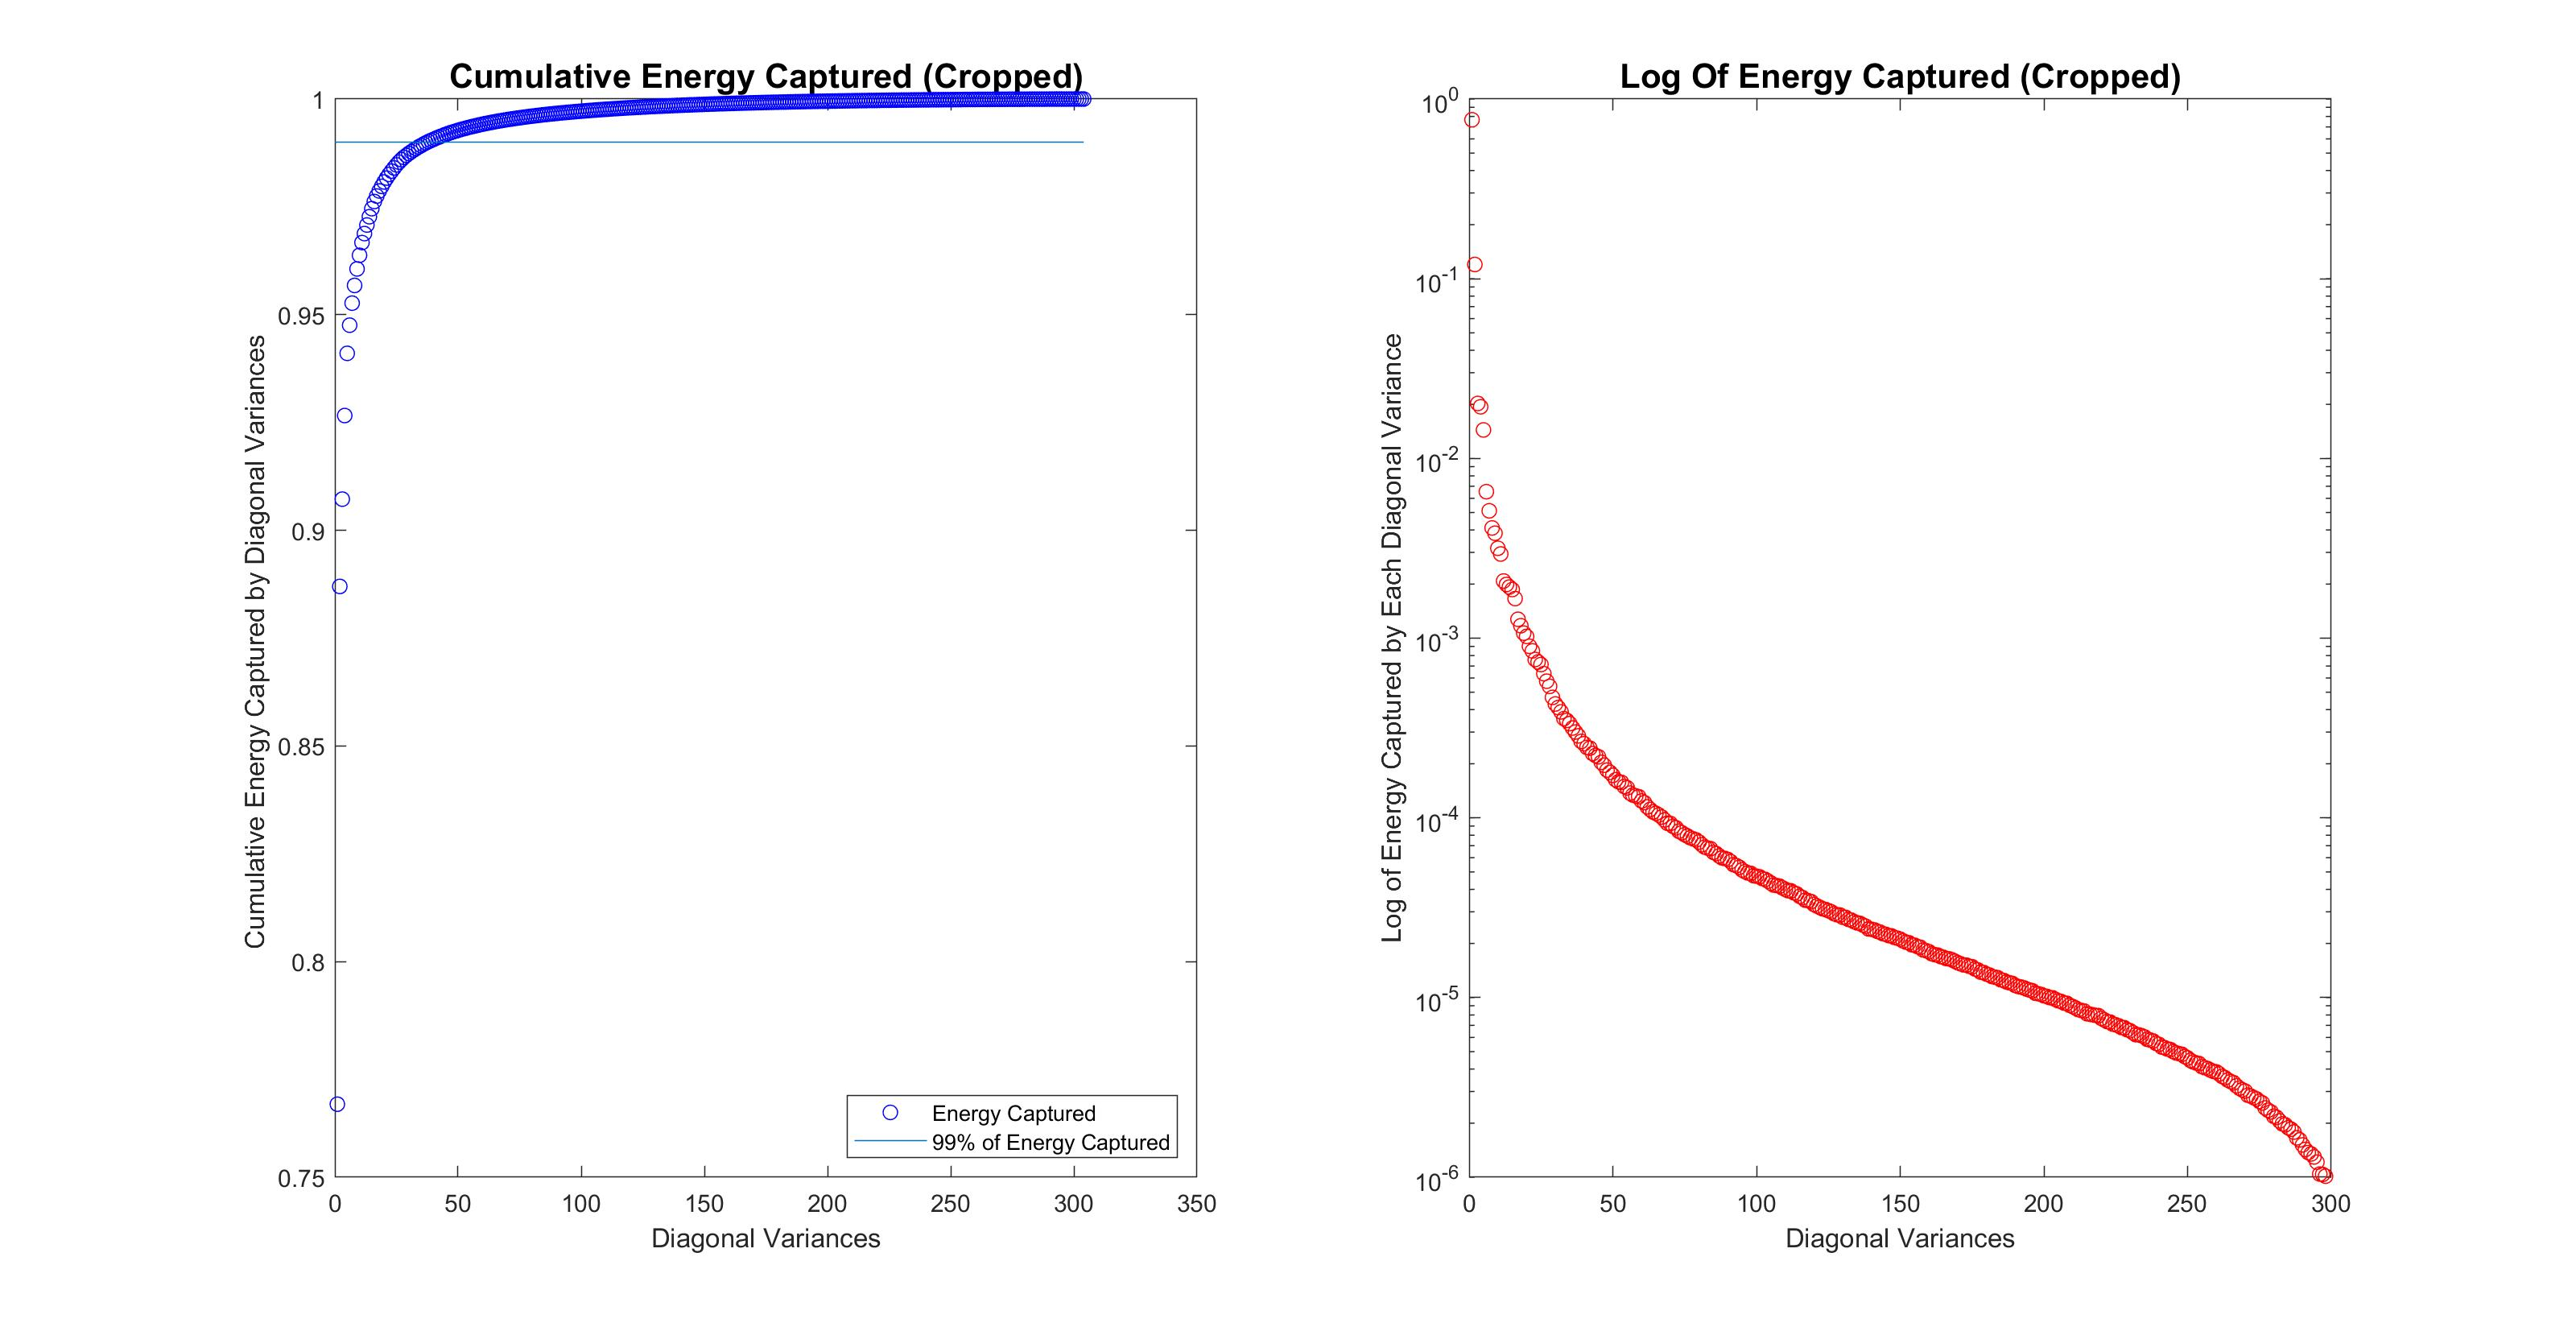
\includegraphics[width = 8cm]{var1}
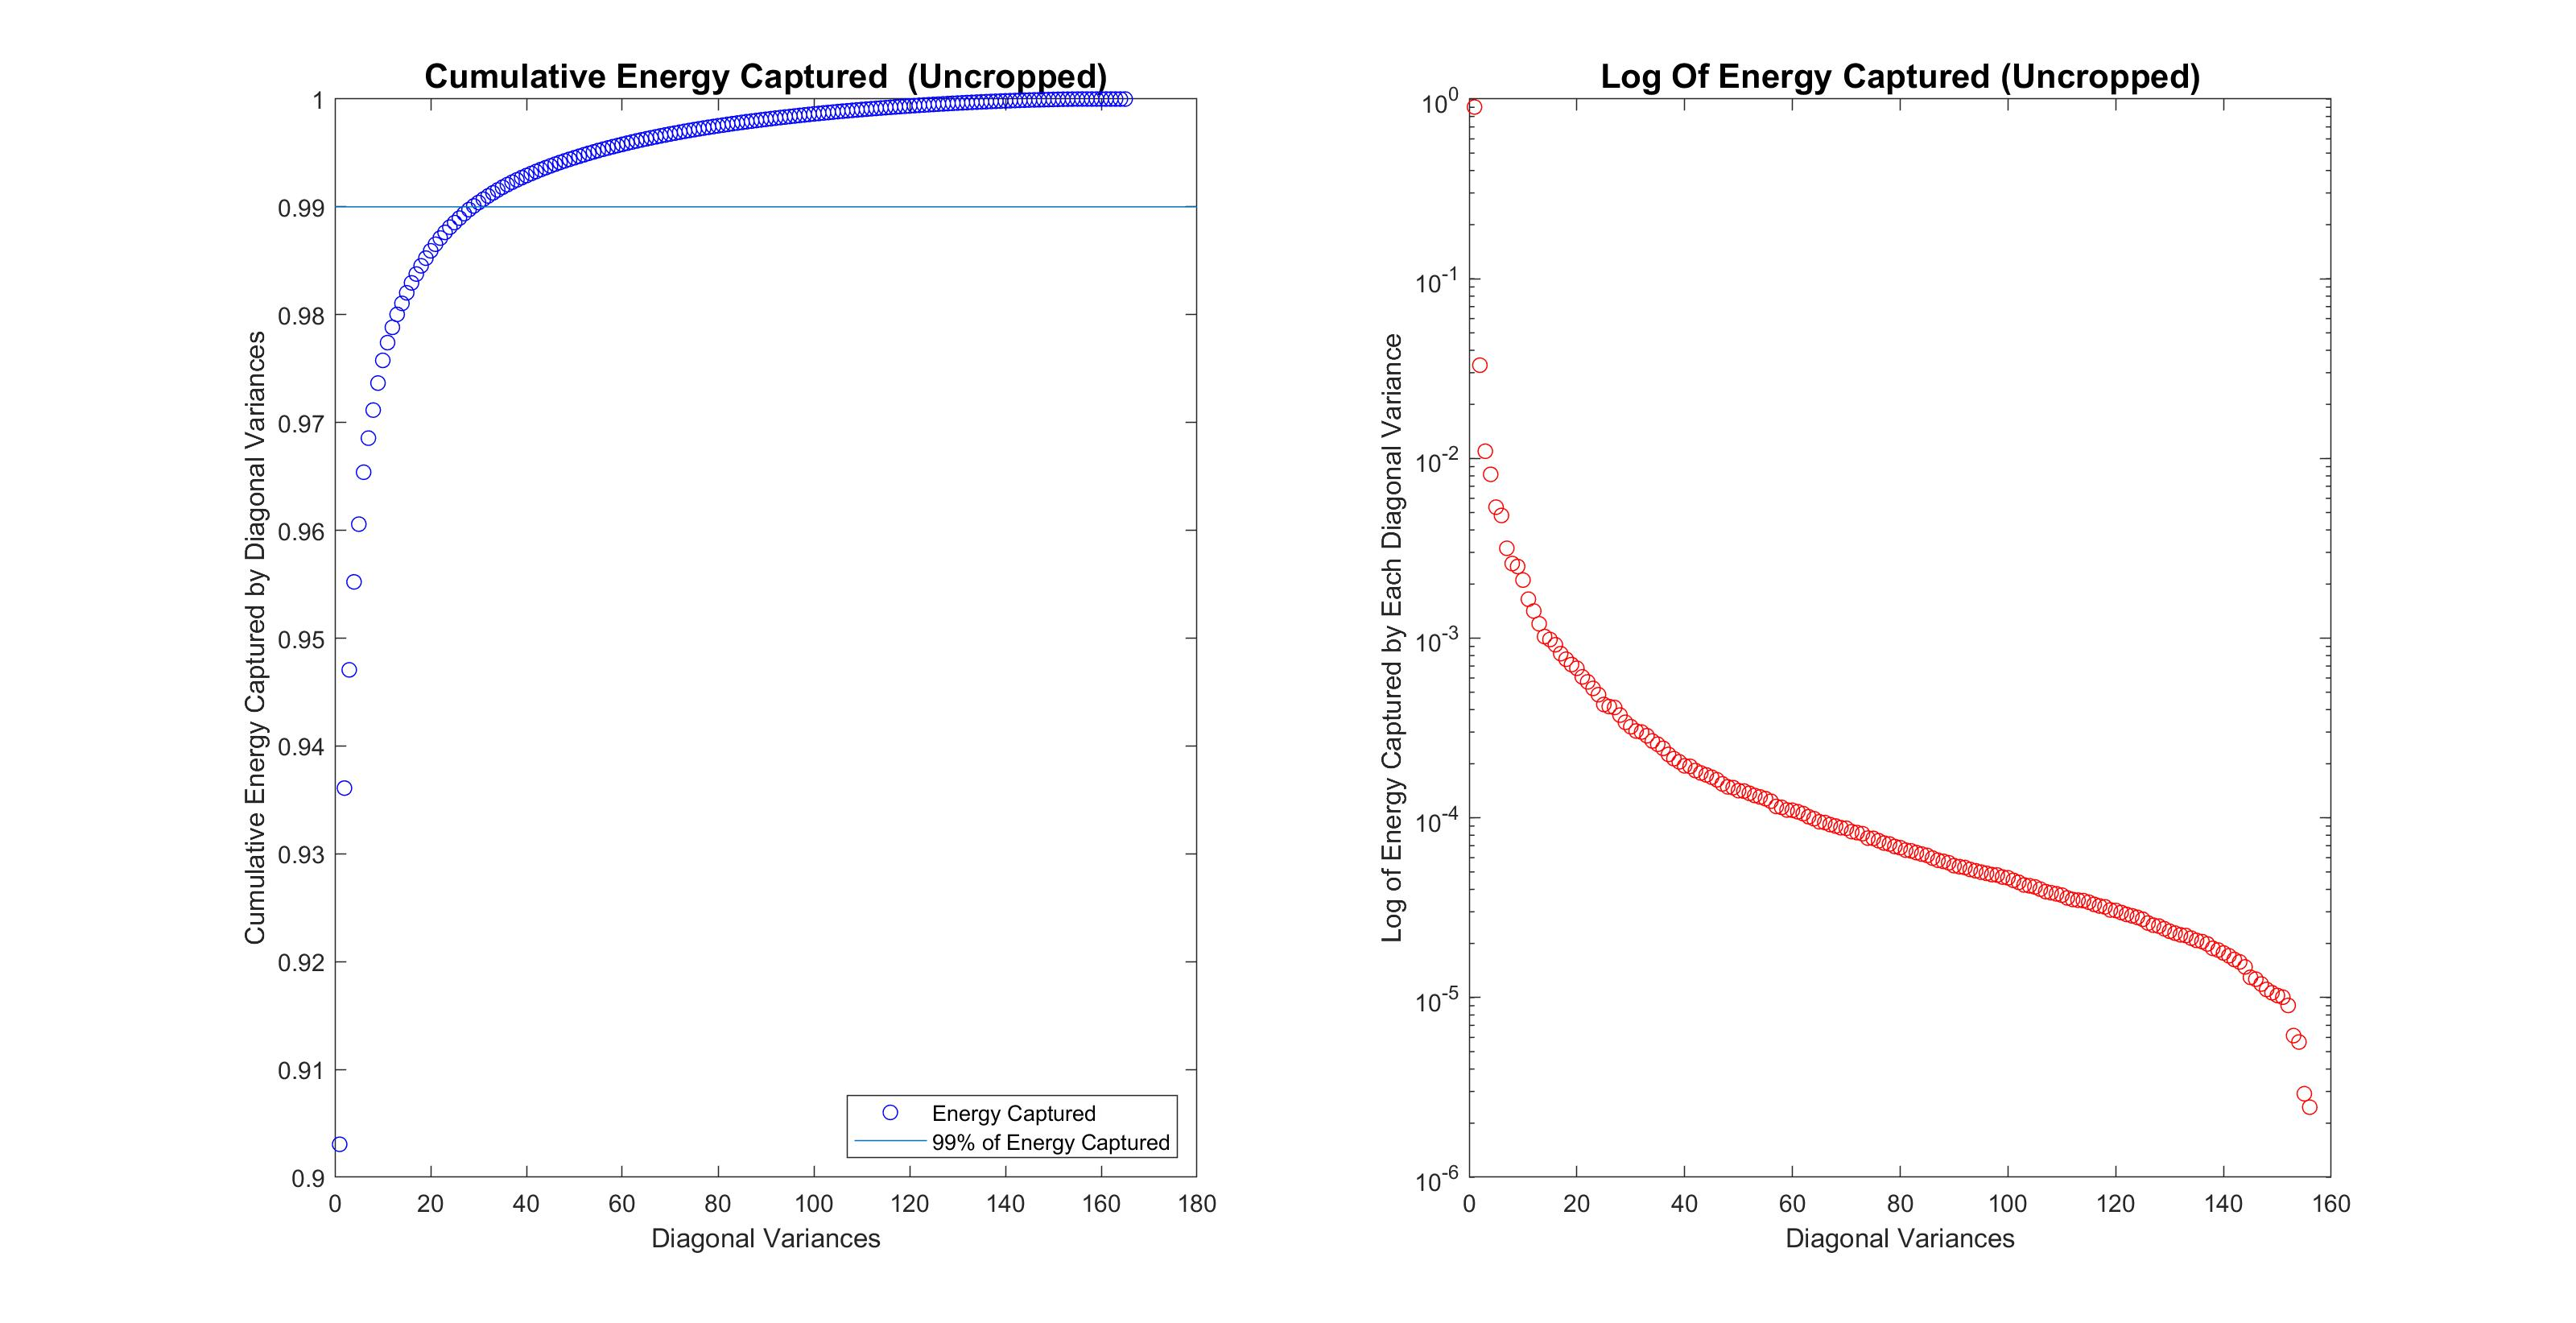
\includegraphics[width = 8cm]{var2}
\caption{ Plots of energy for cropped (left) and uncropped (right)}
\end{center}
\end{figure}

\begin{figure}[H]
\begin{center}
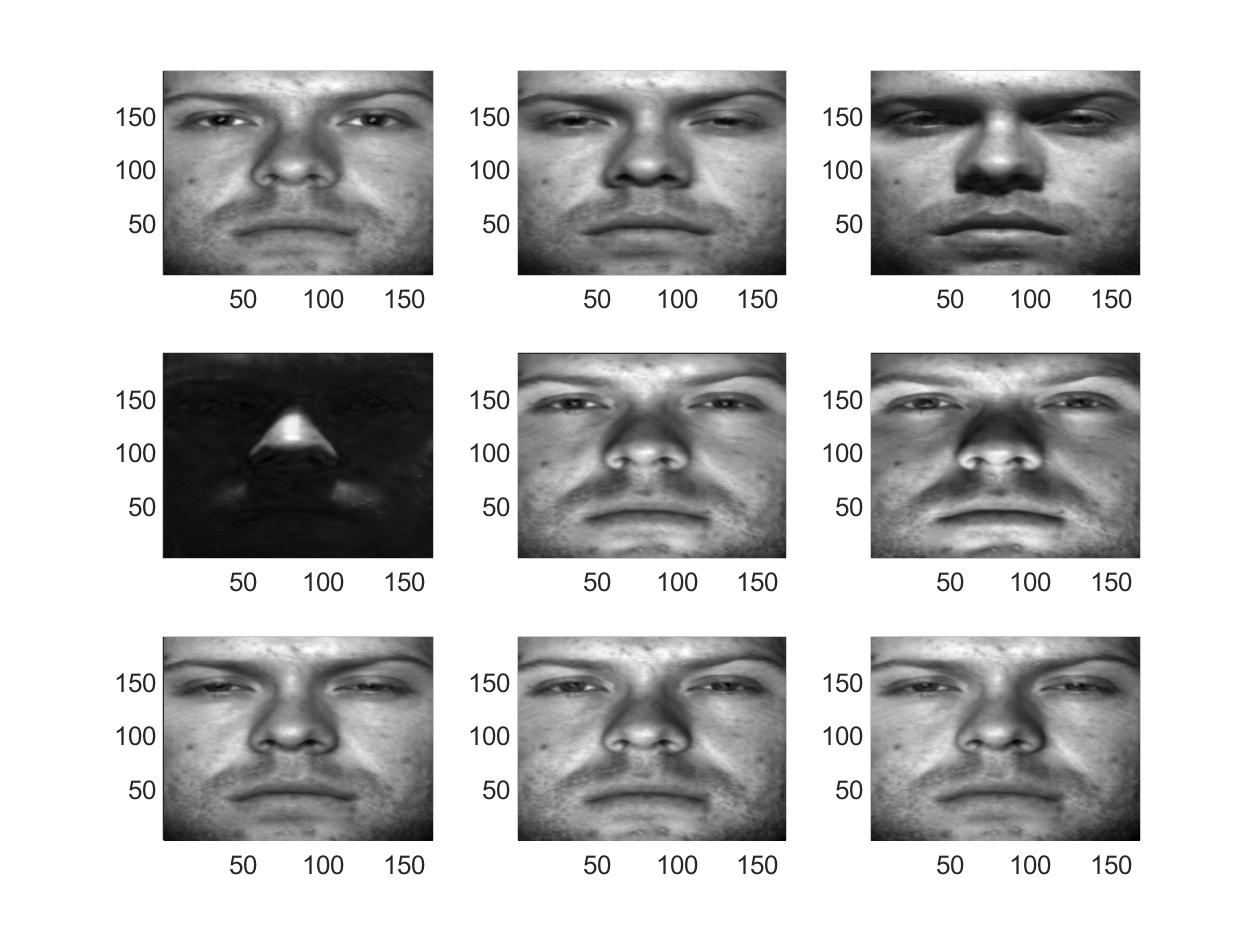
\includegraphics[width = 8cm]{crop}
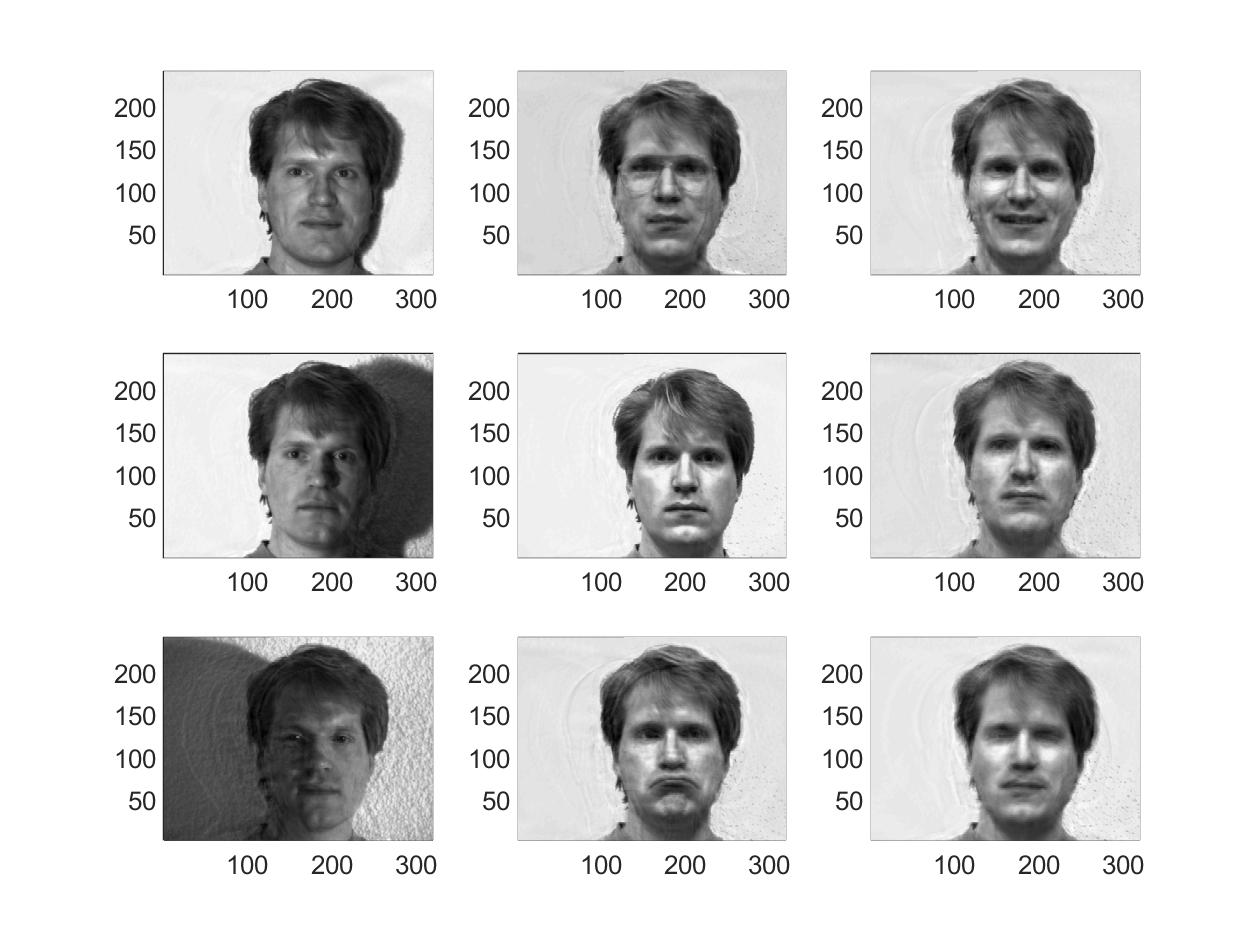
\includegraphics[width = 8cm]{uncrop}
\caption{ Plots of energy for cropped (left) and uncropped (right)}
\end{center}
\end{figure}
We looked at the energy diagrams for both sets of images to reconstruct them with a lower rank. For the uncropped images, we found that a rank of 108 was sufficient enough to convey 99.9\% of the energy. For the cropped images, we found this value to be 160. We were able to come up with clear reconstructions of the data, as shown in the above images. We see that the rank of the face space is 108 and 160 respectively for uncropped and cropped. In our SVD decomposition, our U is the eigenface space. This means that our U*S is our weighted eigen face; they are the "modes" or the basis vectors in n-dimensional space. The S matrix tells us how strong each of these vectors explains the variance; how important each of these principal components are to our data. Finally, V gives the coefficients for each of the data point's projection into the new basis; the ith column of the V matrix represents the coefficients of linear combinations in which we add U*S to get the ith face back. We see that compared to the cropped faces, the uncropped faces do not need as many singular modes to reconstruct the data at a high energy level. \\ \\
	\textbf{Part 2: Music Classification} \\ \\
\begin{figure}[H]
\begin{center}
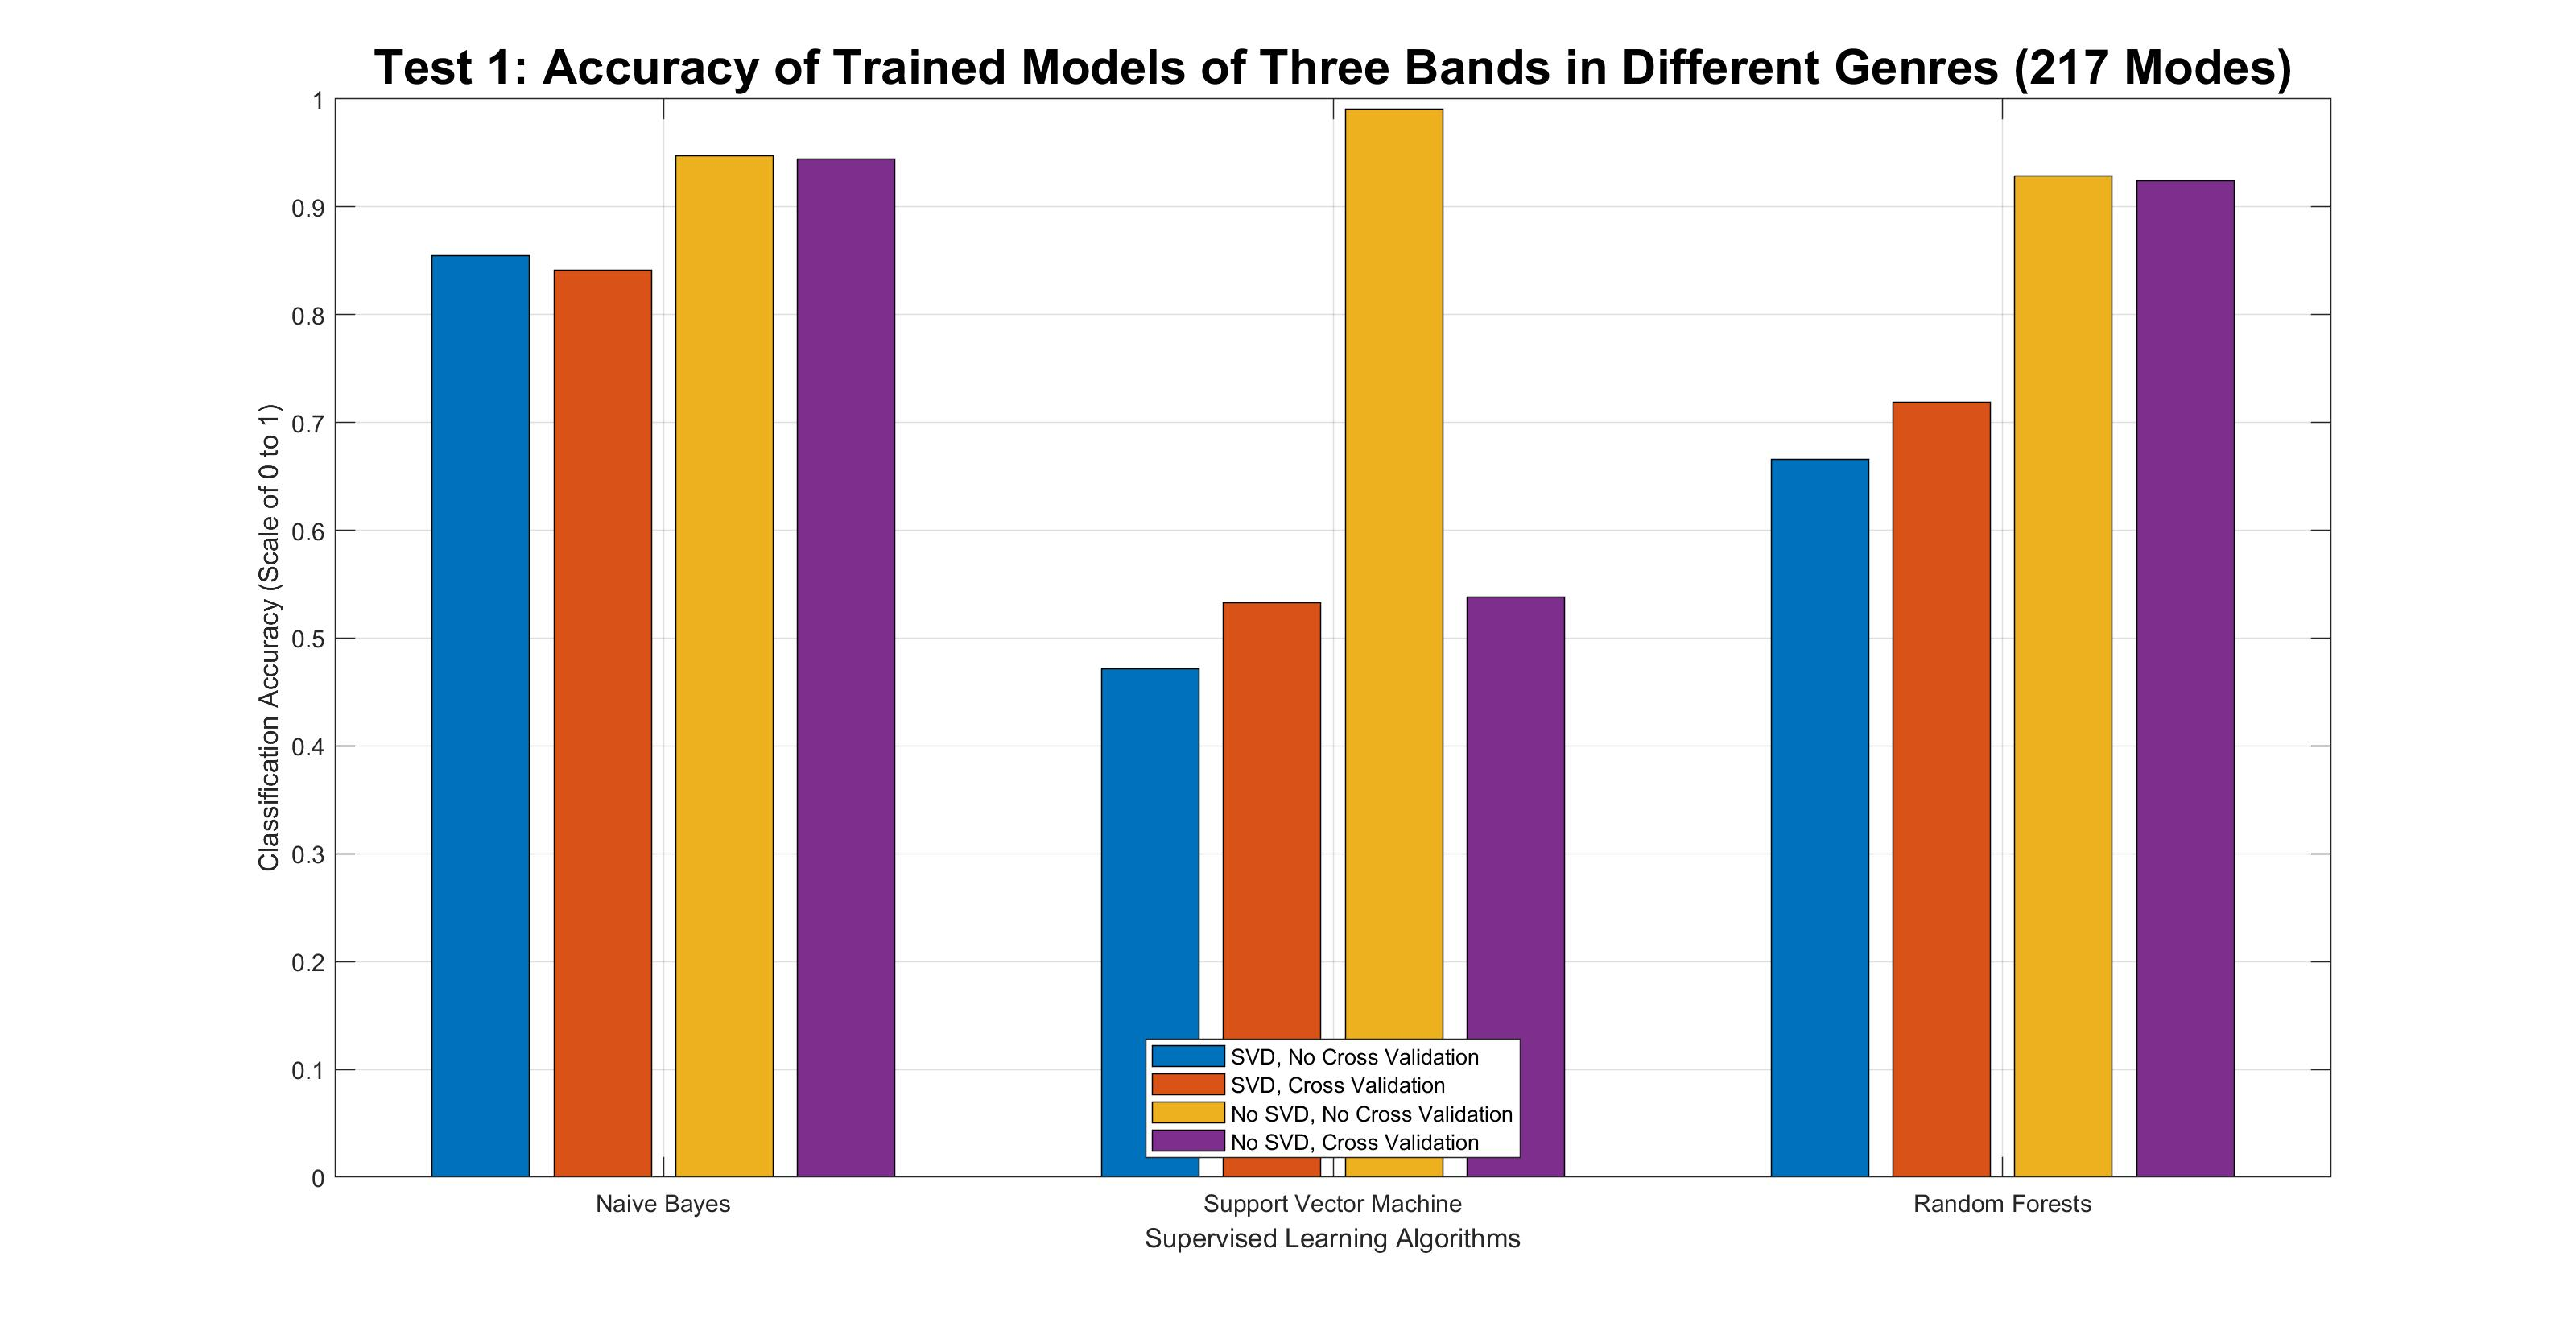
\includegraphics[width = 16cm]{acc1}
\caption{\label{fig:scaled_diss}  Plots of accuracy of supervised learning algorithms (test 1)}
\end{center}
\end{figure}
\begin{figure}[H]
\begin{center}
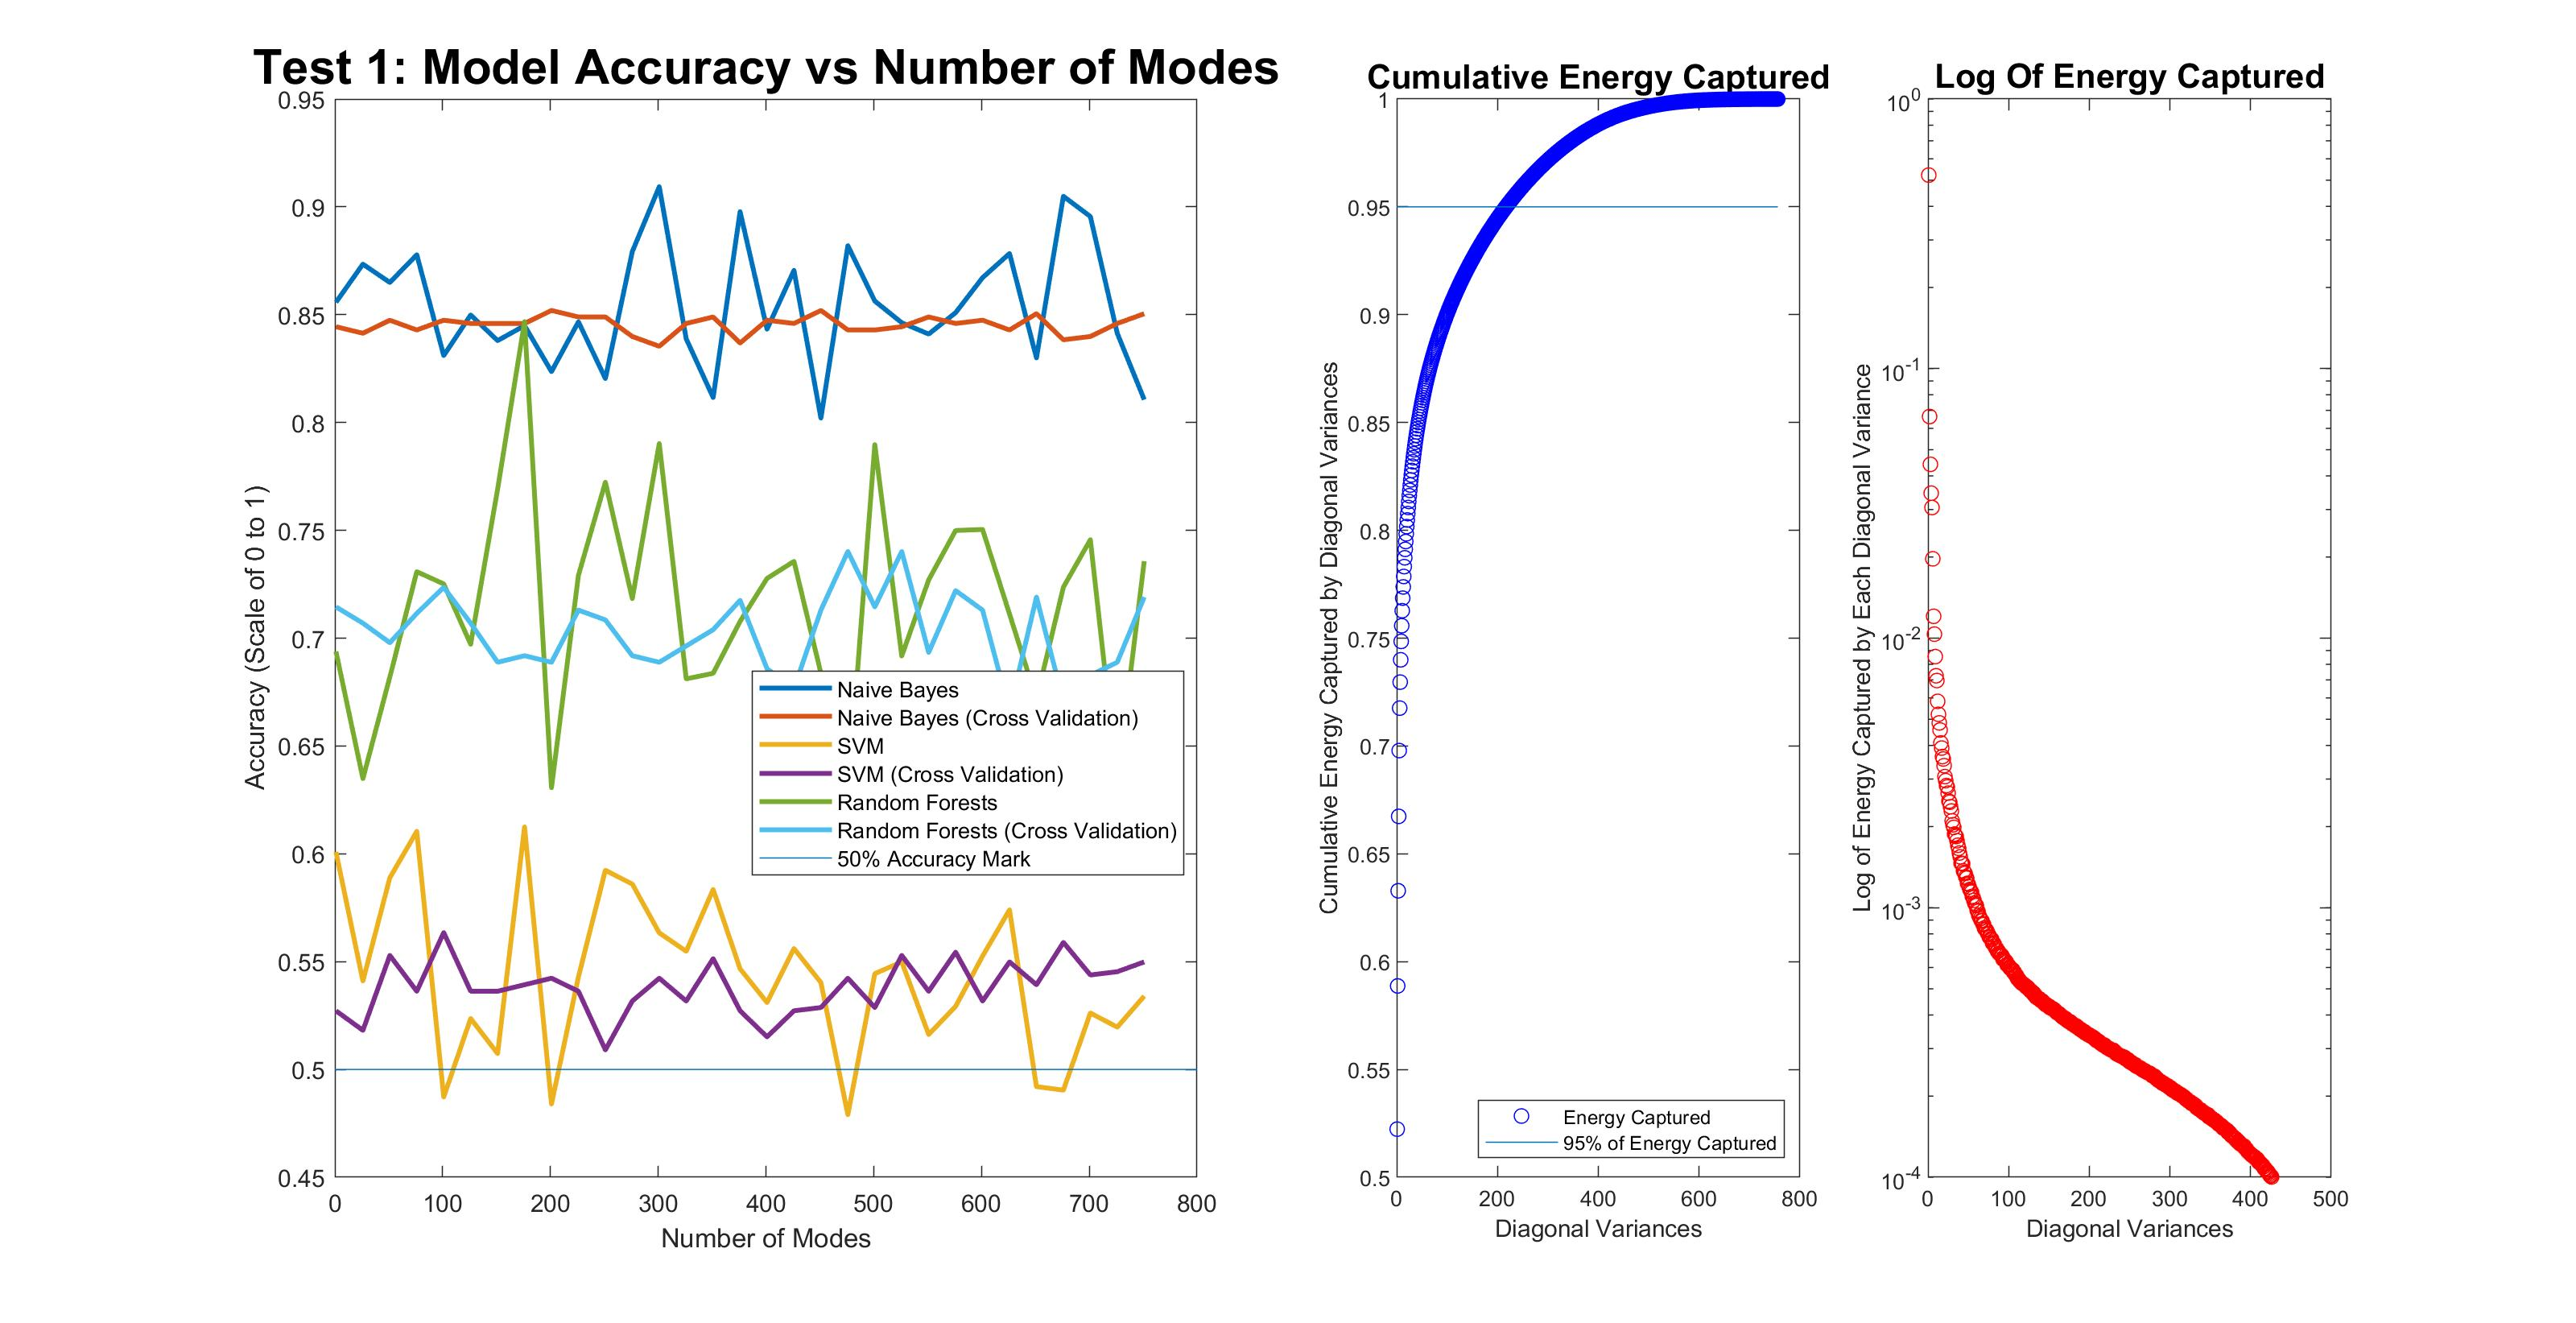
\includegraphics[width = 18cm]{use1}
\caption{\label{fig:scaled_diss} Plots of energy (right) and accuracy with variable mode number (left)  (test 1) }
\end{center}
\end{figure}
	\textbf{Test 1: Band Classification}
	We saw that we were able to capture 95\% of energy with 217 modes, as shown in Figure 4, so we used this number for our truncation of our "u" matrix.. We then compared the prediction accuracy of each of the models, as shown in Figure 3. We see that Naive Bayes performed remarkably well on non cross validated and cross validated data. For SVD, it had 88.73\% and 84.14\% accuracy respectively, and for non SVD, 95.16\% and 94.26\% percent accuracy. We see that with SVM, with SVD, it had low classifcation accuracies of non cross validated and cross validated data, both under 45\%, while for the non SVD data in these categories, it had a 97.06\% classification and 54.08\% classification. We see that there is a large descrepancy in SVM's accuracy of this non SVD data; it has high classification accuracy for non-cross validated, but not for cross-validated. For RF, we observed somewhat high accuracies for the SVD data (0.7760 and 0.6692 for n-cv and cv), and very high accuracies for both non-cross validated and cross validated non SVD data, both being above 91\%. Figure 4 shows that for SVD data, Naive  Bayes had consistently high accuracy with variable number of modes, followed by random forests and SVM. However, all three models were above the 50\% mark, which shows that they are all competent. \\ \\
\textbf{Test 2: The Case for Seattle}
We saw that we were able to capture 95\% of energy with 180 modes, as shown in Figure 6. Figure 5 shows the relative accuracies for each of our models. For NB, we saw that it did not perform well on the SVD data, with accuracies near or slightly below 0.5, for non-crossvalidated and cross-validated cases. However, for the non SVD data, it performed well for both cross-validated and non-cross validated, with accuracies of 87.26\% and 84.64\% respectively.  We saw similar results with RF; low accuracy (under 0.5) for SVD data, and high (>75\%) accuracy for non SVD data for both cross-validated and non-cross validated. For our SVM, it did not perform well for 3/4 of our tests, with classification under 50\%. However, for the non SVD data with no cross-validation, it had an astonishing 99.01\% accuracy. This was the highest we observed, and was especially impressive due to the general trend of low accuracies for this test case. In addition, Figure 6 shows the huge variability in accuracy in all 6 SVD classification methods by changing the number of modes. Since we were classifying within the same genre, we expect this, because the model should theoretically be worse since there are not as many differences. This is why we see so low classification rates, as well as a huge variability with number of modes. \\ \\
\begin{figure}[H]
\begin{center}
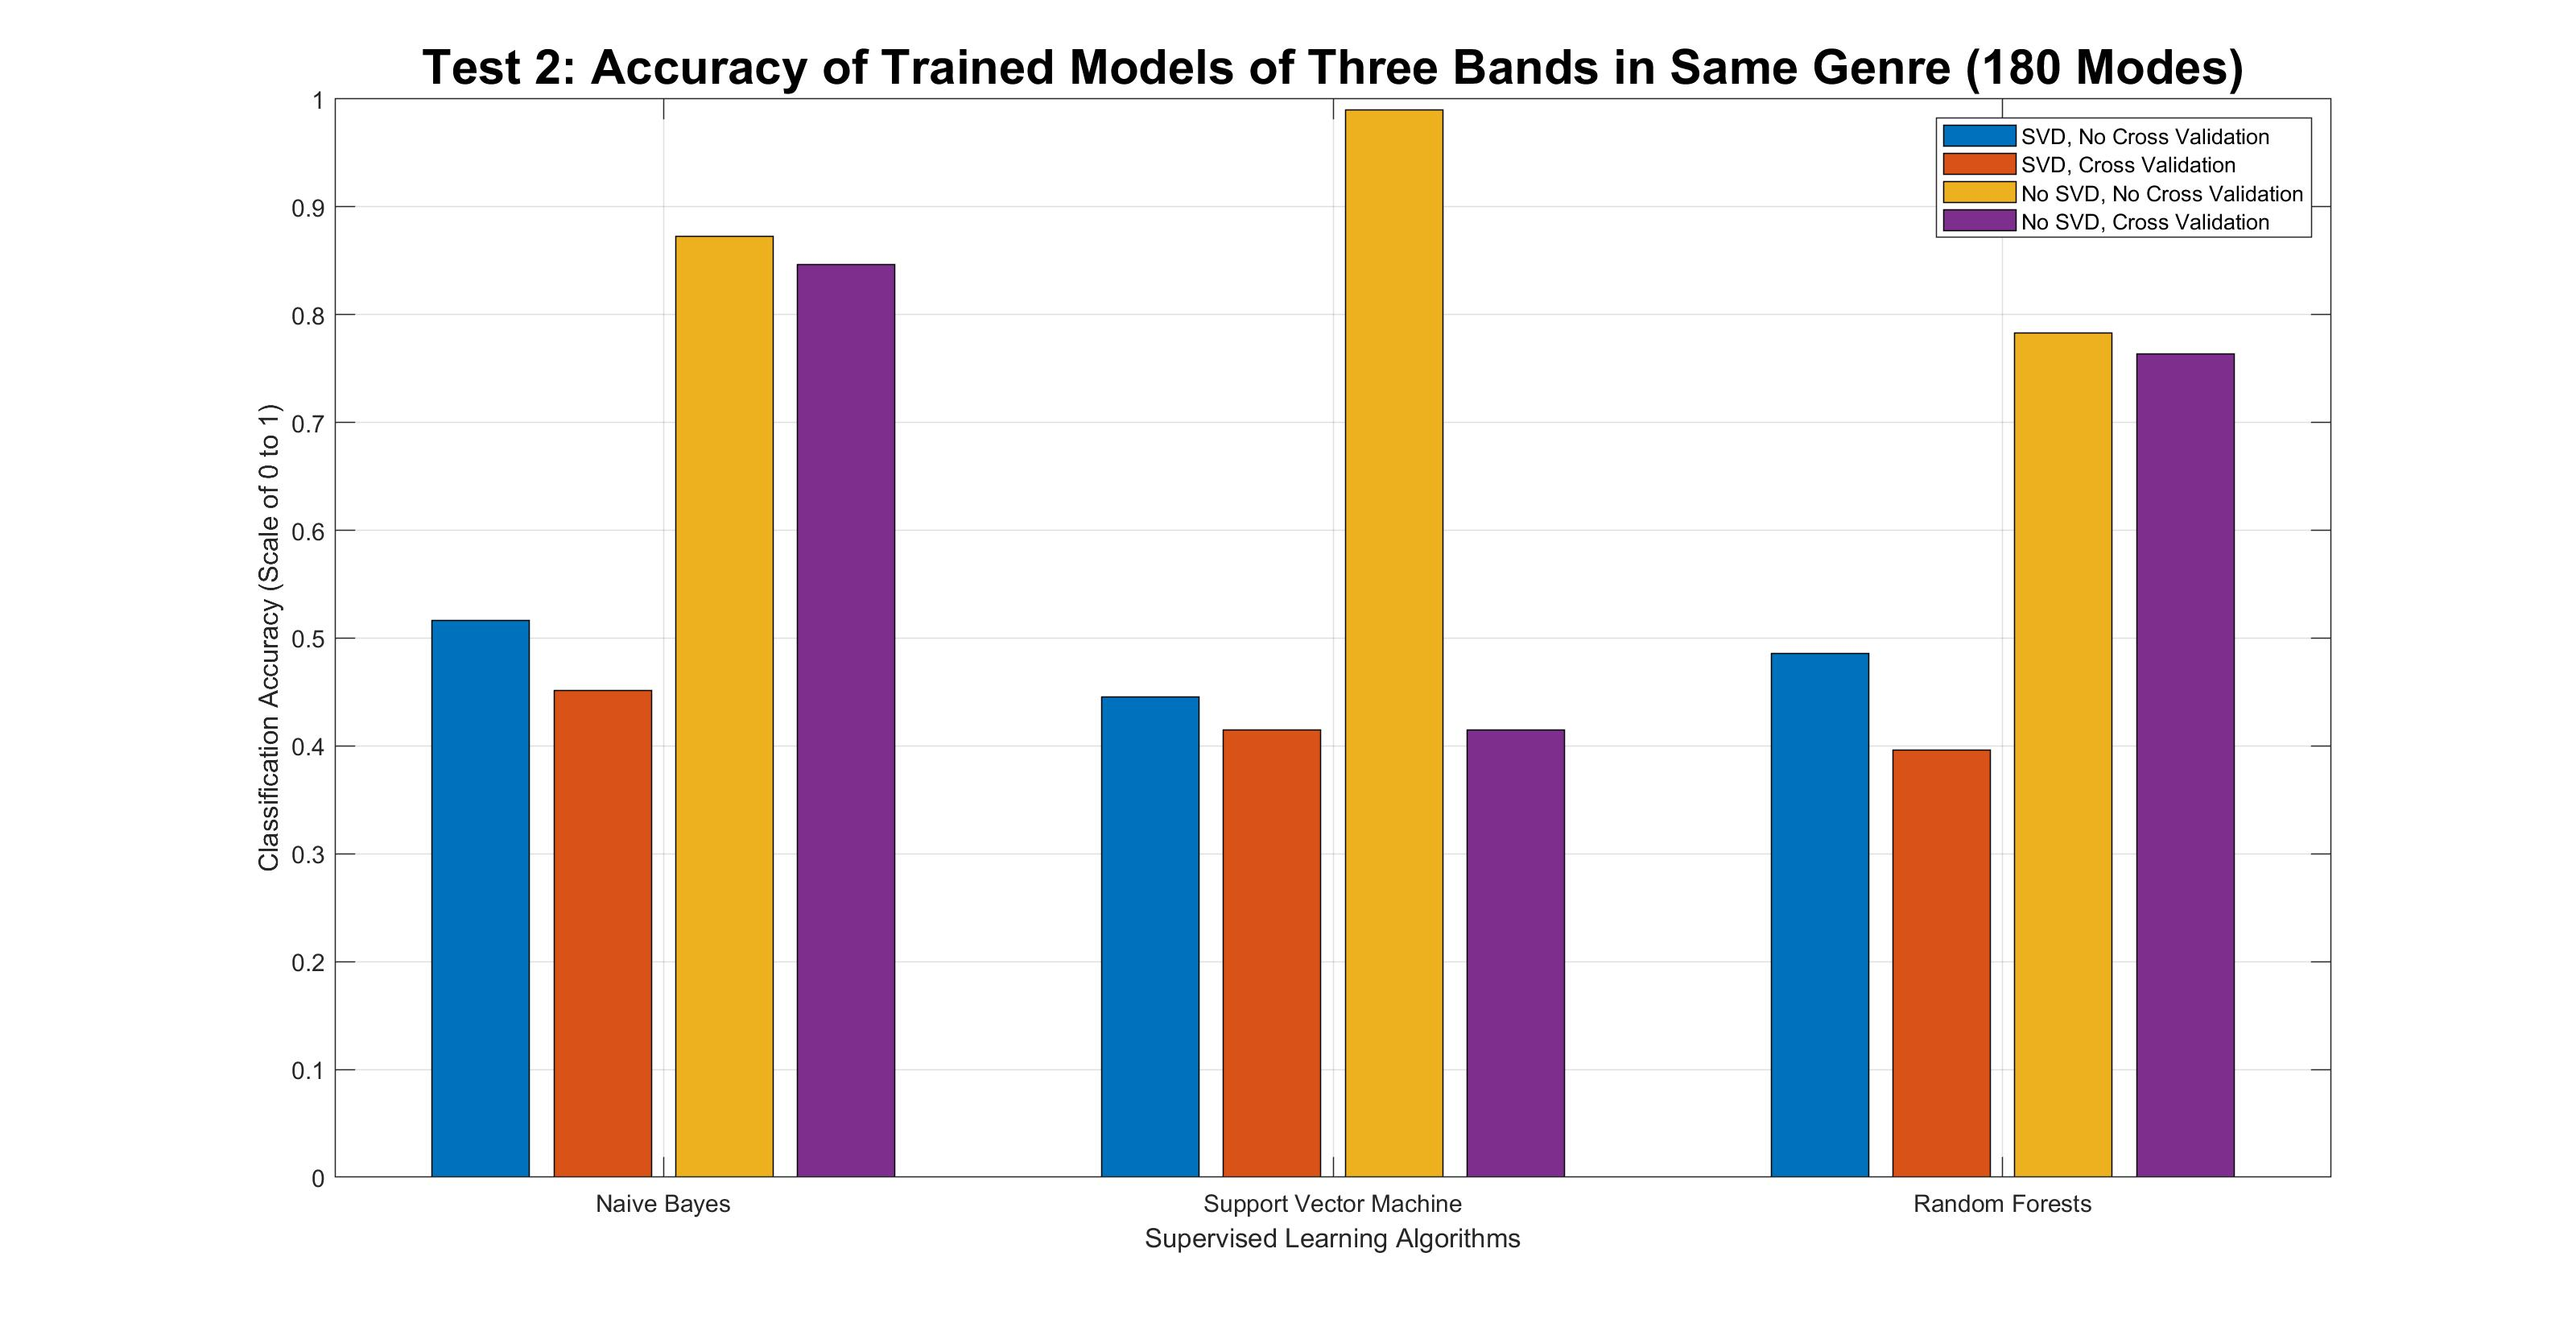
\includegraphics[width = 16cm]{acc2}
\caption{\label{fig:scaled_diss}  Plots of accuracy of supervised learning algorithms (test 2)}
\end{center}
\end{figure}
\begin{figure}[H]
\begin{center}
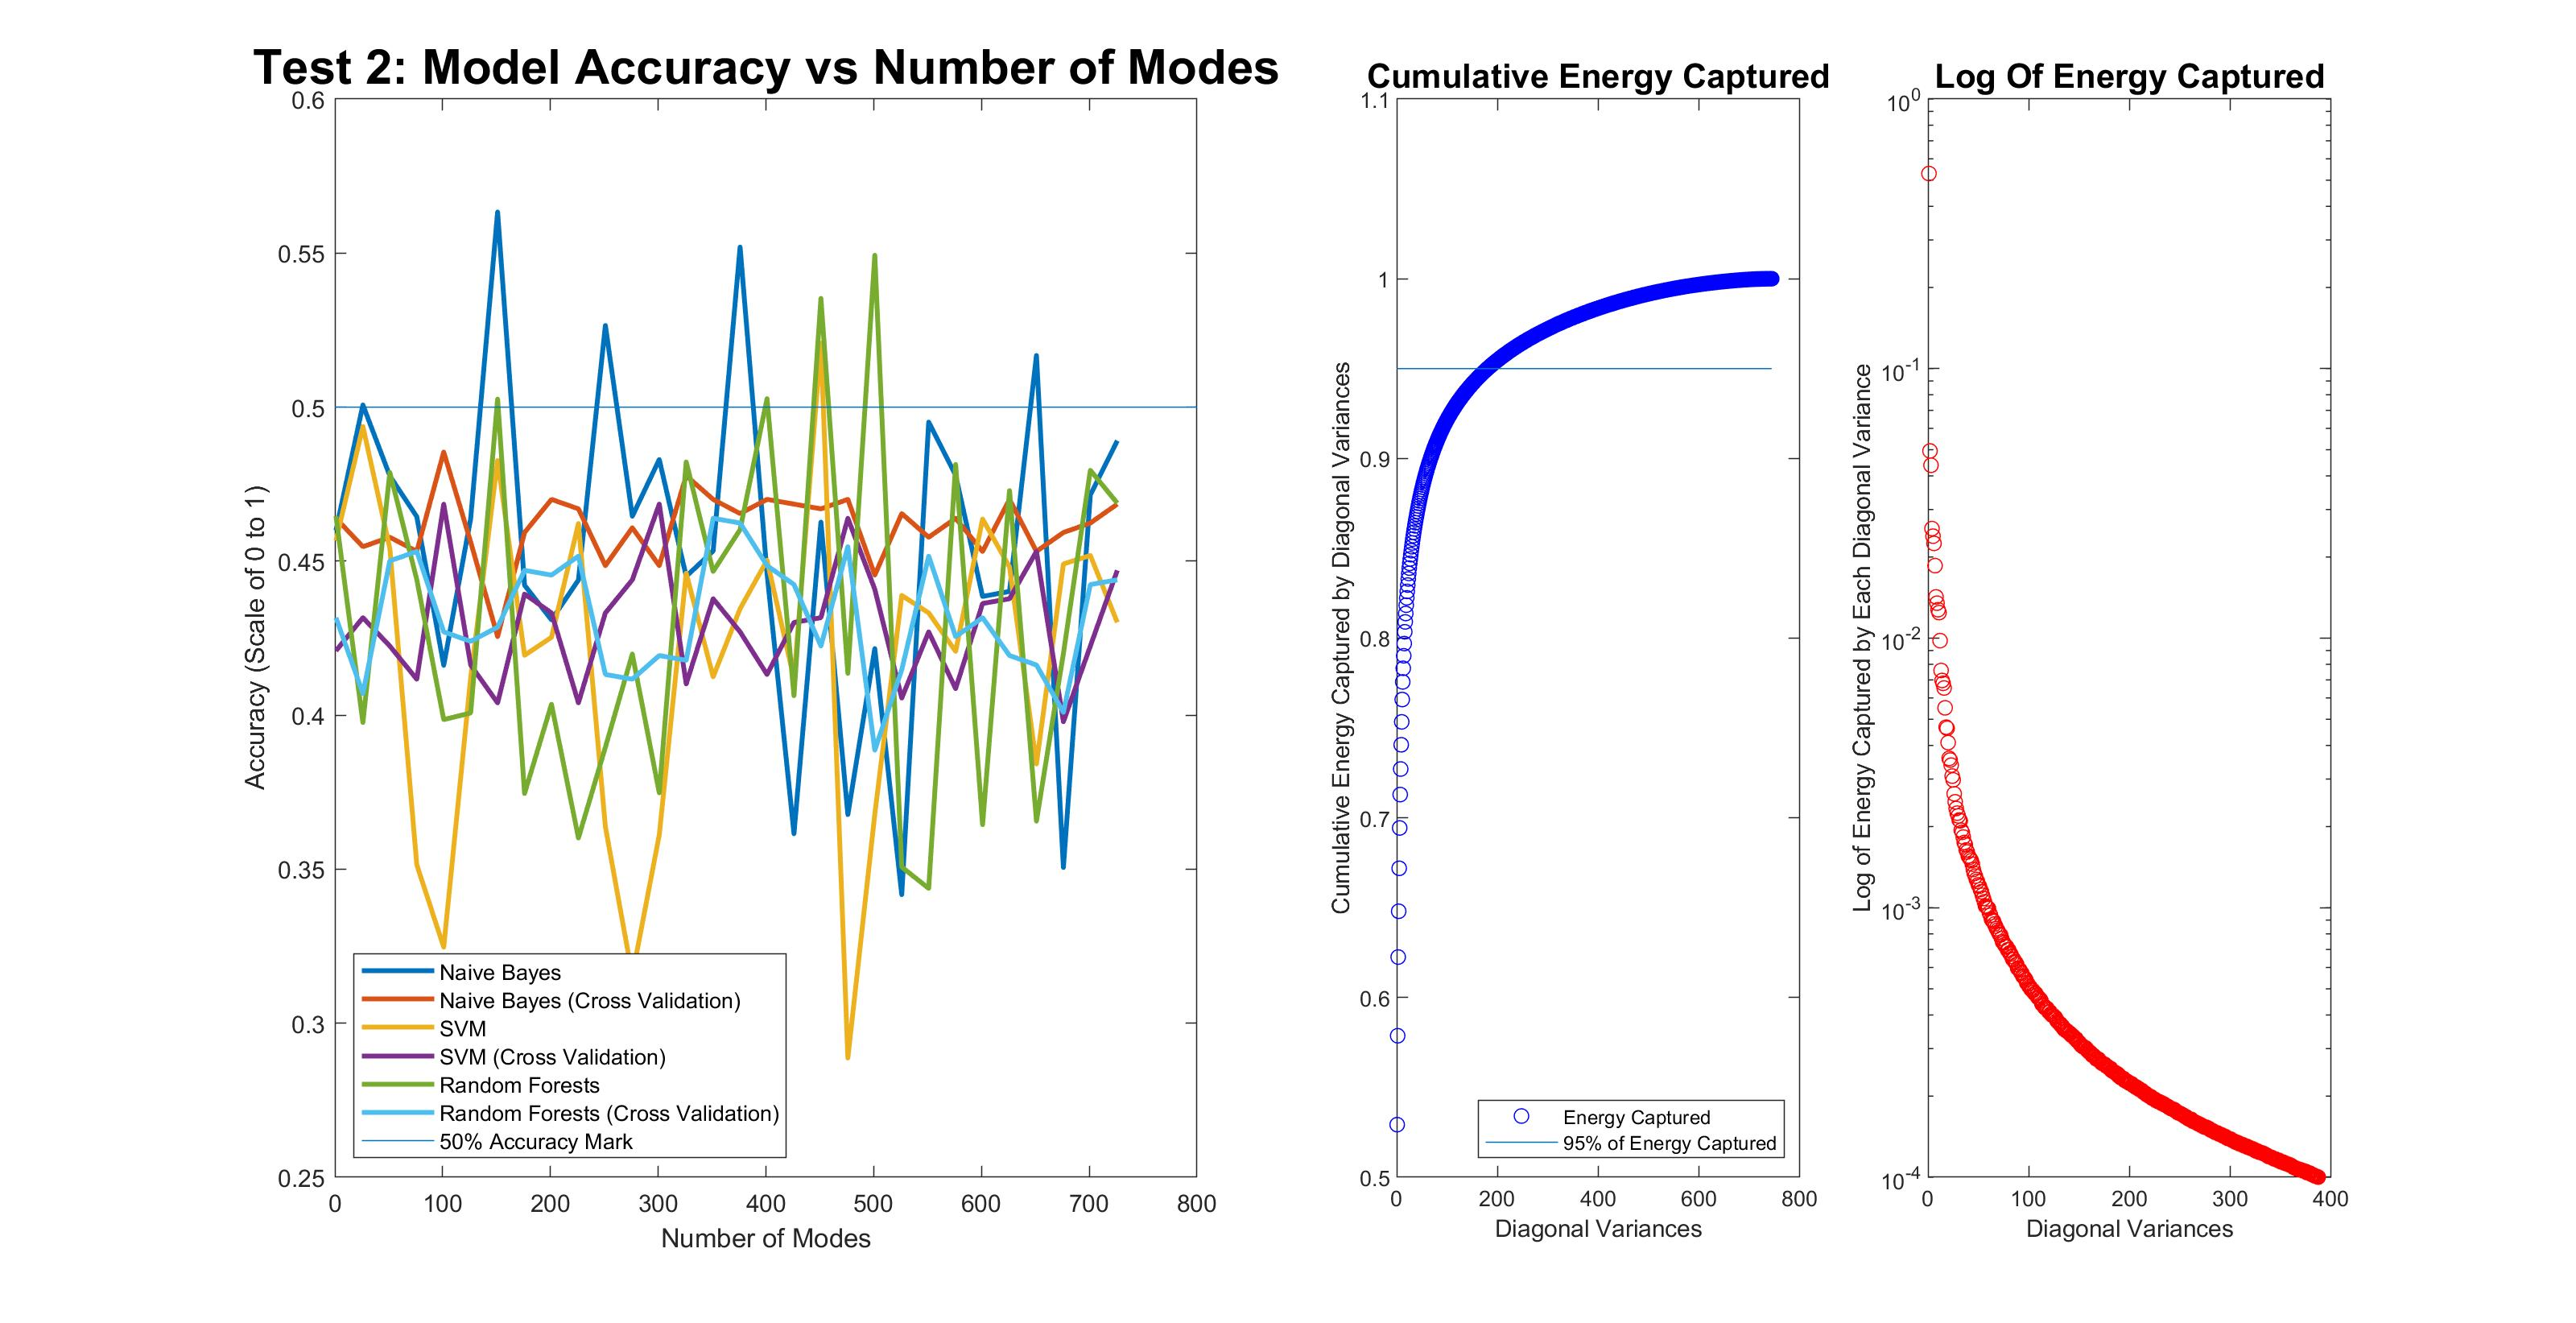
\includegraphics[width = 18cm]{use2}
\caption{\label{fig:scaled_diss} Plots of energy (right) and accuracy with variable mode number (left) (test 2)}
\end{center}
\end{figure}
\textbf{Test 3: Genre Classification}
We found that at 239 modes we were able to represent 95\% of the energy, as shown in Figure 8. In terms of accuracy, all three models (NB, SVM, RF) were not very good at classifying the SVD data, for both non cross-validated cases cross-validated and. For SVM and RF, they had under 50 \% classification for these categories. NB was slightly better with 63.21\% and 64.48\% classification for those categories respectively. Once again, our models were much better at classifying non SVD data: NB was solid with two classification accuracies above 83\% for cross validated and non cross validated, while random forests was slightly worse, with two values above 73\%. Once again, SVM showed strange behavior with the non SVD data: It had remarkbly high classification accuracy of 92.37 \% for the non-cross validated data, and a much lower 45.56\% classification percentage for the cross-validated data. Figure 5 of the accuracies of models on SVD data showed that NB (no cross validation) and NB (cross validation) had consistently high accuracies, depending on the number of nodes, while some models did not perform well at any number, such as both SVM models. Overall, although this graph was less sporadic than Figure 6 for test case 2, there is still some variability, especially compared to test case 1. This shows that it is harder to distinguish between genres when different artists are used, as there is more variability within each genre, since different artists are used. In addition, one reason for the reduced accuracy of this model may be that the genres could have been slightly more similar to eachohter (Rock, Pop, and Motown) than they were in test case 1 (Rap, Classical, Rock). \\ \\
Overall, we found that SVM of non SVD, non cross-validated was consistently accurate for all three test cases. Naive Bayes also had consistently high accuracy for non SVD, in both non cross-validated and cross-validated data, but not as high. We also observe that the SVD classification had much lower accuracy than non SVD data. It makes sense that the non SVD classification had higher accuracy rates, because we are lowering the dimension and feature space with SVD, so we might lose information and accuracy in our model to gain speed (and decrease in computation time). Finally, we note that we had our worst total results in test 2, where we had to distinguish between artists in the same genre. This makes sense because their music will be similar.
\begin{figure}[H]
\begin{center}
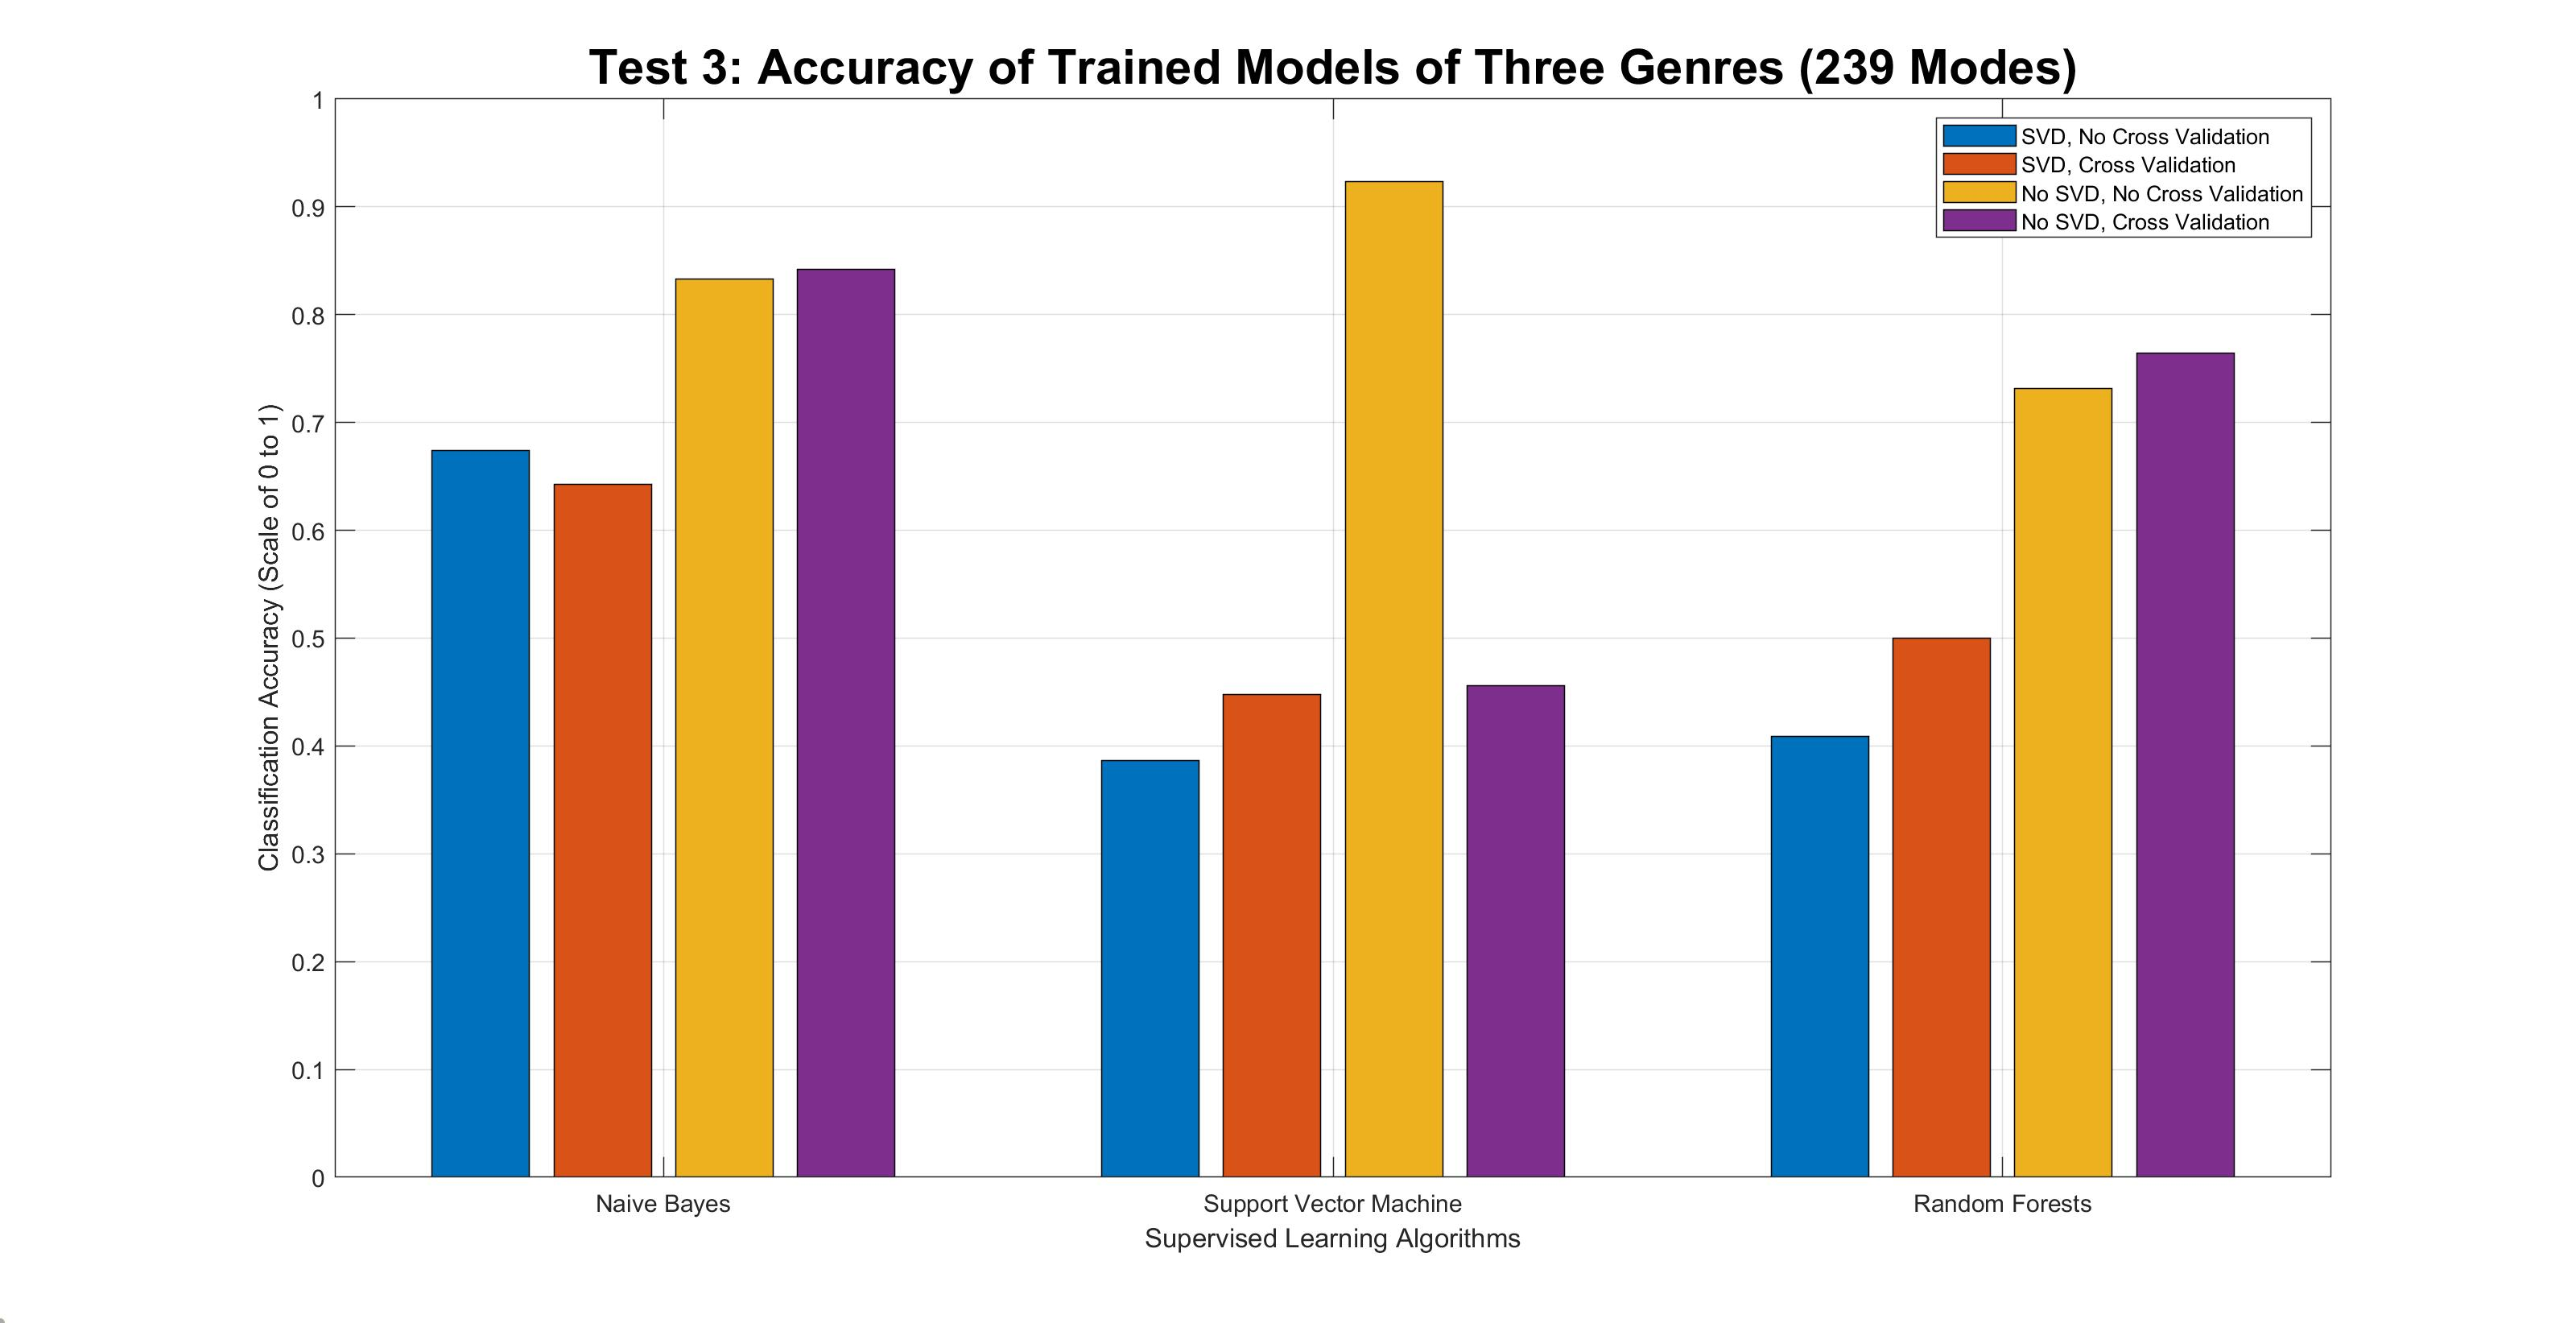
\includegraphics[width = 16cm]{acc3}
\caption{\label{fig:scaled_diss}  Plots of accuracy of supervised learning algorithms (test 3)}
\end{center}
\end{figure}
\begin{figure}[H]
\begin{center}
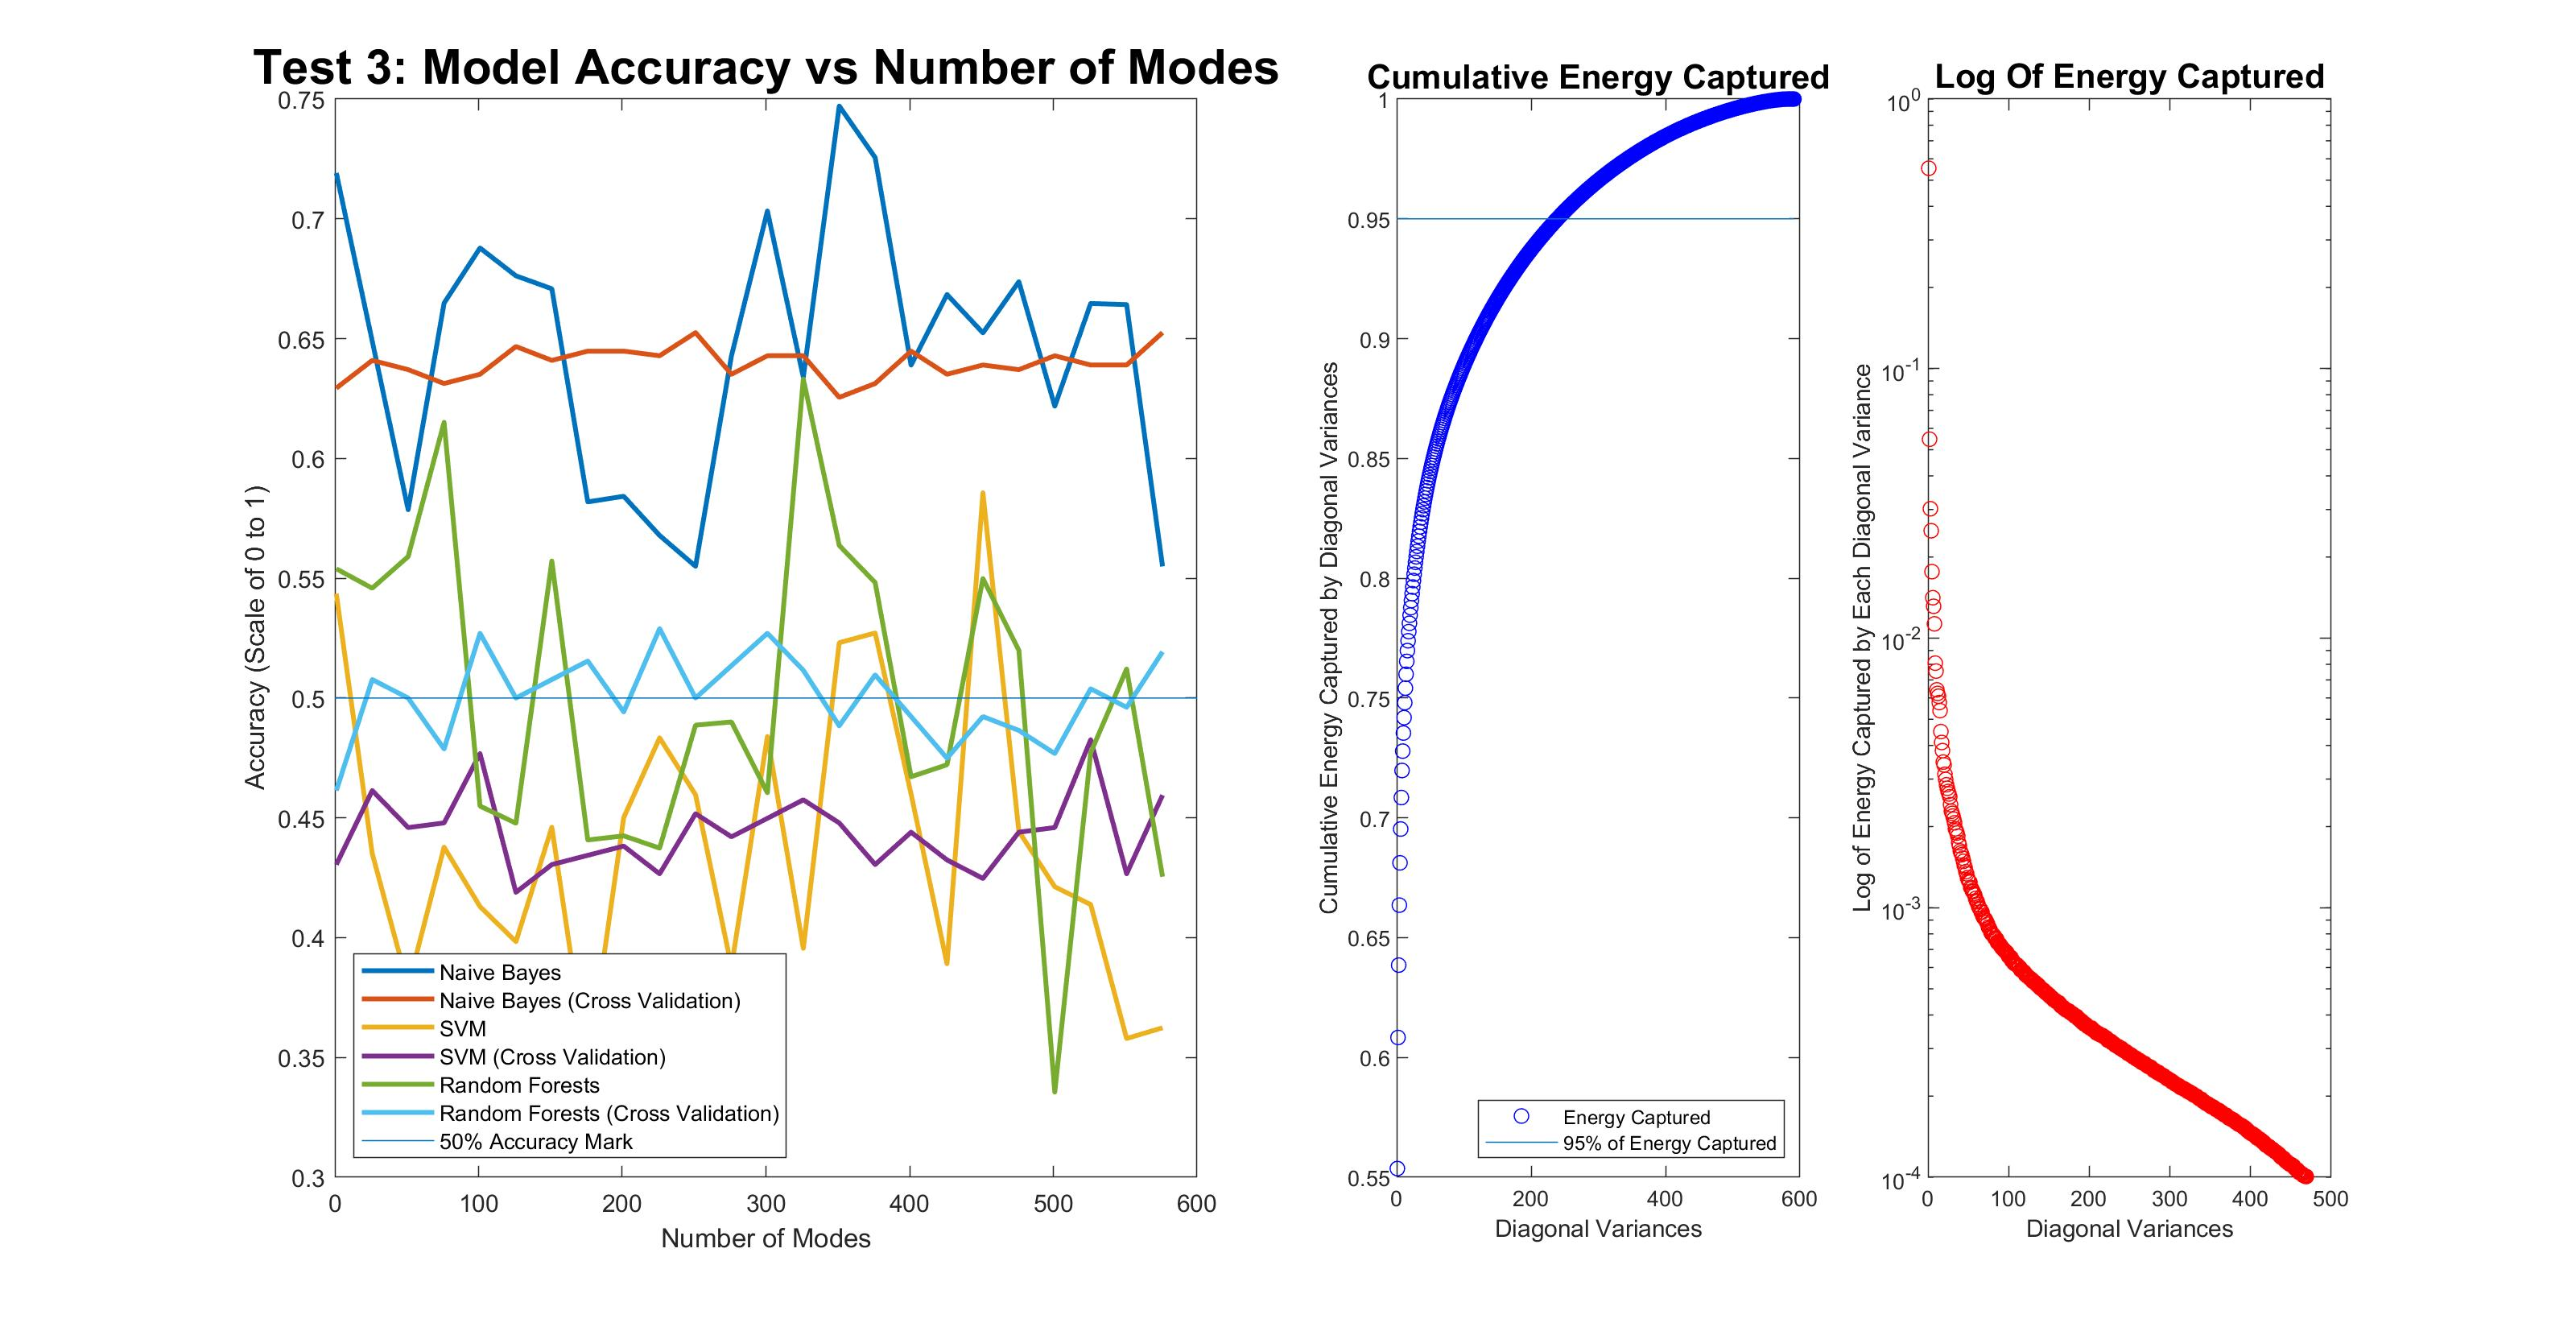
\includegraphics[width = 18cm]{use3}
\caption{\label{fig:scaled_diss} Plots of energy (right) and accuracy with variable mode number (left) (test 3)}
\end{center}
\end{figure}


\section*{\fontsize{19}{15}\selectfont Summary and Conclusions}
In part 1, we were able to perform an SVD across faces and lower the rank after identifying the number of modes that conveyed a lot of the energy. We were then able to reproduce these faces. In part 2, we were able to develop classification models for audio identification using supervised machine learning models. We found that our models performed best when the genres were very different, and the worst when they were the most similar, which is to be expected. In addition, SVM was our best model overall, and non SVD datasets had better classification accuracies than SVD ones.
\pagebreak




\section*{\fontsize{19}{15}\selectfont Appendix A}
\subsection*{MATLAB functions used and implementation}
"audioread(file)": Loads a audio file as one or two vectors (depending on if the file is mono or stereo). We used this to load in our music for classification in part 2. \\
"diag(X)" : Returns a column vector of the diagonal values of a matrix. We used this to generate our variance numbers from SVD. \\ \\
"find(X)" : Returns a vector of non-zero indeces in a matrix. We used this in our conditional matrix to find locations in the image of bright spots, which corresponded to moving object. We then used in "ind2sub" to find direct coordinates.  \\ \\
"fitcnb(data, labels)" : Fits a Naive Bayes Model across the rows of "data", using "labels" to create a model. Can specify cross validation with (..., "crossval", "on") We used this for our music classifcation. \\ \\
"fitcecoc(data, labels)" : Fits a multi-labeled Support Vector Machine with "data", using "labels" to create a model. Can specify cross validation with (..., "crossval", "on") We used this for our music classifcation. \\ \\
"fitctree(data, labels)" : Fits a Random Forests model with "data", using "labels" to create a model. Can specify cross validation with (..., "crossval", "on") We used this for our music classifcation. \\ \\
"floor(x)" : Returns the rounded down integer of a double. We used this to calculate 5 second segments of our sample audio and reshape it. \\ \\
"imread(file)": Reads in an image file as a 3D or 2D matrix (based on if the images is color or grayscale). We used this to load in the Yale Faces for part 1. \\ \\
"kFoldloss(Mdl, data, labels)" : Returns a number between 0 to 1 representing the loss (inaccuracy) of a given cross-volidated model "Mdl", where predicted labels are compared to actual ones ("labels"). We used this to assess the accuracy of our cross validated models. \\ \\
"loss(Mdl, data, labels)" : Returns a number between 0 to 1 representing the loss (inaccuracy) of a given model "Mdl", where predicted labels are compared to actual ones ("labels"). We used this to assess the accuracy of our various models. \\ \\
"max(A)" : If "A" is a vector, then it returns the maximum value of this vector. We used this for normalization of data. \\ \\
"randperm(limit, n)" : Returns a random permutation from 1 to "limit" of size "n". We used this to randomly select training and testing data for model classification. \\ \\
"reshape(A,sz)" : Reshapes the array A to the size "sz". We used this to resize our image matrices into a vector for part 1, and to resize our audio into 5 second segments in part 2. \\ \\
"size(X)" : Returns the dimensions of the matrix "X". We used this to calculate size for audio. \\ \\
"[u,s,v] = svd(X)" : Returns the $U$, $S$, and $V$ matrices corresponded with the singular value decomposition of "X". We used this for the eigen faces in part 1, and for music classification in part 2. \\ \\

\section*{\fontsize{19}{15}\selectfont Appendix B}
\subsection*{MATLAB code}
\begin{lstlisting}[style=Matlab-editor]
clear all; close all; clc; 

close all; clear all; clc;
%% Importing all images from directories (uncropped)
storagestan = [];
Dcy = dir("yalefaces");
for k = 3:length(Dcy)
    data = double(imread(strcat("yalefaces\", Dcy(k).name)));
    storagestan = [storagestan; reshape(data,1,243*320)];
end
%% Importing all images from directories (Cropped)

storagecrop = [];
Dcy = dir("CroppedYale");
for k = 1:length(Dcy)
   curD = Dcy(k).name;
   Dtemp = dir(strcat("CroppedYale\",curD, "\*.pgm"));
   
   for j = 1:length(Dtemp)
       data = double(imread(strcat("CroppedYale\",curD, "\", Dtemp(j).name)));
       storagecrop = [storagecrop; reshape(data,1,192*168)];
   end
end
%% Computation (cropped)
tic
[u,s,v] = svd(storagecrop', 'econ');
toc

%% Plotting and reconstrunction (cropped)
sig = diag(s);
lambda = sig.^2;

subplot(1,2,1)
plot(cumsum(lambda/sum(lambda)), 'bo')
refline(0,0.99)
legend("Energy Captured", "99% of Energy Captured", "Location", "Southeast");
ylabel("Cumulative Energy Captured by Diagonal Variances "); xlabel("Diagonal Variances");
title("Cumulative Energy Captured (Cropped)", "Fontsize", 14);
subplot(1,2,2)
plot(lambda/sum(lambda), 'ro')
set(gca, 'YScale', 'log')
ylim([10e-7, 1]); ylabel("Log of Energy Captured by Each Diagonal Variance"); xlabel("Diagonal Variances");
title("Log Of Energy Captured (Cropped)", "Fontsize", 14);
%% Eigen Faces
reconstruct = u(:,1:160) *s(1:160,:)*v(1:160,:)';
for z = 1:9
    curimg = reshape(reconstruct(:,z), [192,168]);
    subplot(3,3,z);
    pcolor(flip(curimg)), shading interp, colormap(gray)
end


%% NEW PART
tic
[u1,s1,v1] = svd(storagestan', 'econ');
toc

sig1 = diag(s);
lambda1 = sig1.^2;

reconstruct1 = u1(:,1:108) *s1(1:108,:)*v1(1:108,:)';
for z = 1:9
    curimg = reshape(reconstruct1(:,z), [243,320]);
    subplot(3,3,z);
    pcolor(flip(curimg)), shading interp, colormap(gray)
end

sig1 = diag(s1);
lambda1 = sig1.^2;

subplot(1,2,1)
plot(cumsum(lambda1/sum(lambda1)), 'bo')
refline(0,0.99)
legend("Energy Captured", "99% of Energy Captured", "Location", "Southeast");
ylabel("Cumulative Energy Captured by Diagonal Variances"); xlabel("Diagonal Variances");
title("Cumulative Energy Captured  (Uncropped)", "Fontsize", 14);
subplot(1,2,2)
plot(lambda1/sum(lambda1), 'ro')
set(gca, 'YScale', 'log')
ylim([10e-7, 1]); ylabel("Log of Energy Captured by Each Diagonal Variance"); xlabel("Diagonal Variances");
title("Log Of Energy Captured (Uncropped)", "Fontsize", 14);

close all; clear all; clc;

%% Import audio files
alldata = [];
Alabels = [];
for str = {"travi", "billy", "liszt"}
    for i = 1:5
        [song, Fs] = audioread(strcat("Music\",str{1}, num2str(i),".mp3"));
        Fs = Fs/10;

        %Lower sampling rate
        song = song(1:10:end,:);
        
        monosong = [];
        %Convert from stereo to mono
        for z = 1:length(song)
            if (song(z,1) == 0 || song(z,2) == 0)
                monosong(z,1) = max(song(z,:));
            else
                monosong(z,1) = (song(z,1) + song(z,2))/2;
            end
        end


        %Remove leading and trailing 0s
        monosong = monosong(find(monosong,1,'first'):find(monosong,1,'last'));

        %5 second intervals
        chunk_size = Fs*5;

        endpoint = floor(length(monosong) / chunk_size);
        monosong = monosong(1:(chunk_size * endpoint),1);

        data = reshape(monosong, [chunk_size, endpoint]);
        alldata = [alldata, data];
        Alabels = [Alabels; repmat(str{1}, size(data,2) ,1)];
    end
end
Alabels = Alabels.';
traindata = alldata;
trainlabels = Alabels;
%% Rearrange and apply fft
[u,s,v] = svd(abs(fft(alldata)), 'econ');
trainlabels = Alabels;

sig = diag(s);
lambda = sig.^2;

utrunc = u(:, 1:217);
traindata = utrunc'*alldata;

n = floor(size(traindata, 2)/(8));
c = randperm(size(traindata,2), n);
    
testdata = traindata(:,c);
testlabels = trainlabels(:,c);

traindata(:,c) = [];
trainlabels(:,c) = [];

nosvdtraindata = abs(fft(alldata));
nosvdtestdata = nosvdtraindata(:,c);
nosvdtraindata(:,c) = [];
%% Modeling
nbMdl = fitcnb(traindata.', trainlabels);
nbL = loss(nbMdl, testdata.', testlabels)

%Cross validation model
nbcvMdl = fitcnb(traindata.', trainlabels, 'crossval', 'on');
nbcvL = kfoldLoss(nbcvMdl,'LossFun','ClassifErr')

svmMdl = fitcecoc(traindata.', trainlabels);
svmL = loss(svmMdl, testdata.', testlabels)

%Cross validation model
svmcvMdl = fitcecoc(traindata.', trainlabels, 'crossval', 'on');
svmcvL = kfoldLoss(svmcvMdl,'LossFun','ClassifErr')

rfMdl = fitctree(traindata.', trainlabels);
rfL = loss(rfMdl, testdata.', testlabels)

%Cross validation model
rfcvMdl = fitctree(traindata.', trainlabels, 'crossval', 'on');
rfcvL = kfoldLoss(rfcvMdl,'LossFun','ClassifErr')

%% Modeling (no SVD)
nosvdnbMdl = fitcnb(nosvdtraindata.', trainlabels);
nosvdnbL = loss(nosvdnbMdl, nosvdtestdata.', testlabels)

%Cross validation model
nosvdnbcvMdl = fitcnb(nosvdtraindata.', trainlabels, 'crossval', 'on');
nosvdnbcvL = kfoldLoss(nosvdnbcvMdl,'LossFun','ClassifErr')

nosvdsvmMdl = fitcecoc(nosvdtraindata.', trainlabels);
nosvdsvmL = loss(nosvdsvmMdl, nosvdtestdata.', testlabels)

%Cross validation model
nosvdsvmcvMdl = fitcecoc(traindata.', trainlabels, 'crossval', 'on');
nosvdsvmcvL = kfoldLoss(nosvdsvmcvMdl,'LossFun','ClassifErr')

nosvdrfMdl = fitctree(nosvdtraindata.', trainlabels);
nosvdrfL = loss(nosvdrfMdl, nosvdtestdata.', testlabels)

%Cross validation model
nosvdrfcvMdl = fitctree(nosvdtraindata.', trainlabels, 'crossval', 'on');
nosvdrfcvL = kfoldLoss(nosvdrfcvMdl,'LossFun','ClassifErr')

%% Plotting
close all;

bar(1-[nbL nbcvL nosvdnbL nosvdnbcvL; svmL svmcvL nosvdsvmL nosvdsvmcvL; rfL rfcvL nosvdrfL nosvdrfcvL])
xticklabels(["Naive Bayes", "Support Vector Machine", "Random Forests"]);
legend("SVD, No Cross Validation", "SVD, Cross Validation", "No SVD, No Cross Validation", "No SVD, Cross Validation",...
    "Location", "south");
ylabel("Classification Accuracy (Scale of 0 to 1)"); xlabel("Supervised Learning Algorithms");
title("Test 1: Accuracy of Trained Models of Three Bands in Different Genres (217 Modes)", 'FontSize', 20);
grid on

%% Loop
tic
classify= []
for z = 1:25:size(u,2)
    trunc = u(:, 1:z);
    traindata = utrunc'*alldata;
    trainlabels = Alabels;
    
    n = floor(size(traindata, 2)/(8));
    c = randperm(size(traindata,2), n);
    
    testdata = traindata(:,c);
    testlabels = trainlabels(:,c);
    traindata(:,c) = [];
    trainlabels(:,c) = [];
    
    nbMdl = fitcnb(traindata.', trainlabels);
    nbcvMdl = fitcnb(traindata.', trainlabels, 'crossval', 'on');

    svmMdl = fitcecoc(traindata.', trainlabels);
    svmcvMdl = fitcecoc(traindata.', trainlabels, 'crossval', 'on');

    rfMdl = fitctree(traindata.', trainlabels);
    rfcvMdl = fitctree(traindata.', trainlabels, 'crossval', 'on');
    
    classify= [classify; loss(nbMdl, testdata.', testlabels) , kfoldLoss(nbcvMdl,'LossFun','ClassifErr'), ...
                       loss(svmMdl, testdata.', testlabels), kfoldLoss(svmcvMdl,'LossFun','ClassifErr'), ...
                        loss(rfMdl, testdata.', testlabels), kfoldLoss(rfcvMdl,'LossFun','ClassifErr')];
                    
end
toc

%% Plot bigger stuff
close all;

subplot(1,2,1)
plot(1:25:size(u,2), 1-classify, "Linewidth", 2)
title("Test 1: Model Accuracy vs Number of Modes", "Fontsize", 20);
xlabel("Number of Modes"); ylabel("Accuracy (Scale of 0 to 1)");
refline(0,0.5)
legend("Naive Bayes", "Naive Bayes (Cross Validation)", "SVM", "SVM (Cross Validation)", ...
    "Random Forests", "Random Forests (Cross Validation)","50% Accuracy Mark", "Location", "best");

subplot(1,4,3)
plot(cumsum(lambda/sum(lambda)), 'bo')
refline(0,0.95)
legend("Energy Captured", "95% of Energy Captured", "Location", "Southeast");
ylabel("Cumulative Energy Captured by Diagonal Variances"); xlabel("Diagonal Variances");
title("Cumulative Energy Captured", "Fontsize", 14);
subplot(1,4,4)
plot(lambda/sum(lambda), 'ro')
set(gca, 'YScale', 'log')
ylim([10e-5, 1]); ylabel("Log of Energy Captured by Each Diagonal Variance"); xlabel("Diagonal Variances");
title("Log Of Energy Captured", "Fontsize", 14);

close all; clear all; clc;

%% Import audio files
alldata = [];
Alabels = [];
for str = {"drake", "travi", "migos"}
    for i = 1:5
        [song, Fs] = audioread(strcat("Music\",str{1}, num2str(i),".mp3"));
        Fs = Fs/10;

        %Lower sampling rate
        song = song(1:10:end,:);
        
        monosong = [];
        %Convert from stereo to mono
        for z = 1:length(song)
            if (song(z,1) == 0 || song(z,2) == 0)
                monosong(z,1) = max(song(z,:));
            else
                monosong(z,1) = (song(z,1) + song(z,2))/2;
            end
        end


        %Remove leading and trailing 0s
        monosong = monosong(find(monosong,1,'first'):find(monosong,1,'last'));

        %5 second intervals
        chunk_size = Fs*5;

        endpoint = floor(length(monosong) / chunk_size);
        monosong = monosong(1:(chunk_size * endpoint),1);

        data = reshape(monosong, [chunk_size, endpoint]);
        alldata = [alldata, data];
        Alabels = [Alabels; repmat(str{1}, size(data,2) ,1)];
    end
end
Alabels = Alabels.';
traindata = alldata;
trainlabels = Alabels;
%% Rearrange and apply fft
[u,s,v] = svd(abs(fft(alldata)), 'econ');
trainlabels = Alabels;

sig = diag(s);
lambda = sig.^2;

utrunc = u(:, 1:180);
traindata = utrunc'*alldata;

n = floor(size(traindata, 2)/(8));
c = randperm(size(traindata,2), n);
    
testdata = traindata(:,c);
testlabels = trainlabels(:,c);

traindata(:,c) = [];
trainlabels(:,c) = [];

nosvdtraindata = abs(fft(alldata));
nosvdtestdata = nosvdtraindata(:,c);
nosvdtraindata(:,c) = [];
%% Modeling
nbMdl = fitcnb(traindata.', trainlabels);
nbL = loss(nbMdl, testdata.', testlabels)

%Cross validation model
nbcvMdl = fitcnb(traindata.', trainlabels, 'crossval', 'on');
nbcvL = kfoldLoss(nbcvMdl,'LossFun','ClassifErr')

svmMdl = fitcecoc(traindata.', trainlabels);
svmL = loss(svmMdl, testdata.', testlabels)

%Cross validation model
svmcvMdl = fitcecoc(traindata.', trainlabels, 'crossval', 'on');
svmcvL = kfoldLoss(svmcvMdl,'LossFun','ClassifErr')

rfMdl = fitctree(traindata.', trainlabels);
rfL = loss(rfMdl, testdata.', testlabels)

%Cross validation model
rfcvMdl = fitctree(traindata.', trainlabels, 'crossval', 'on');
rfcvL = kfoldLoss(rfcvMdl,'LossFun','ClassifErr')

%% Modeling (no SVD)
nosvdnbMdl = fitcnb(nosvdtraindata.', trainlabels);
nosvdnbL = loss(nosvdnbMdl, nosvdtestdata.', testlabels)

%Cross validation model
nosvdnbcvMdl = fitcnb(nosvdtraindata.', trainlabels, 'crossval', 'on');
nosvdnbcvL = kfoldLoss(nosvdnbcvMdl,'LossFun','ClassifErr')

nosvdsvmMdl = fitcecoc(nosvdtraindata.', trainlabels);
nosvdsvmL = loss(nosvdsvmMdl, nosvdtestdata.', testlabels)

%Cross validation model
nosvdsvmcvMdl = fitcecoc(traindata.', trainlabels, 'crossval', 'on');
nosvdsvmcvL = kfoldLoss(nosvdsvmcvMdl,'LossFun','ClassifErr')

nosvdrfMdl = fitctree(nosvdtraindata.', trainlabels);
nosvdrfL = loss(nosvdrfMdl, nosvdtestdata.', testlabels)

%Cross validation model
nosvdrfcvMdl = fitctree(nosvdtraindata.', trainlabels, 'crossval', 'on');
nosvdrfcvL = kfoldLoss(nosvdrfcvMdl,'LossFun','ClassifErr')

%% Plotting
close all;

bar(1-[nbL nbcvL nosvdnbL nosvdnbcvL; svmL svmcvL nosvdsvmL nosvdsvmcvL; rfL rfcvL nosvdrfL nosvdrfcvL])
xticklabels(["Naive Bayes", "Support Vector Machine", "Random Forests"]);
legend("SVD, No Cross Validation", "SVD, Cross Validation", "No SVD, No Cross Validation", "No SVD, Cross Validation");
ylabel("Classification Accuracy (Scale of 0 to 1)"); xlabel("Supervised Learning Algorithms");
title("Test 2: Accuracy of Trained Models of Three Bands in Same Genre (180 Modes)", 'FontSize', 20);
grid on
%% Loop
tic
classify= []
for z = 1:25:size(u,2)
    trunc = u(:, 1:z);
    traindata = utrunc'*alldata;
    trainlabels = Alabels;
    
    n = floor(size(traindata, 2)/(8));
    c = randperm(size(traindata,2), n);
    
    testdata = traindata(:,c);
    testlabels = trainlabels(:,c);
    traindata(:,c) = [];
    trainlabels(:,c) = [];
    
    nbMdl = fitcnb(traindata.', trainlabels);
    nbcvMdl = fitcnb(traindata.', trainlabels, 'crossval', 'on');

    svmMdl = fitcecoc(traindata.', trainlabels);
    svmcvMdl = fitcecoc(traindata.', trainlabels, 'crossval', 'on');

    rfMdl = fitctree(traindata.', trainlabels);
    rfcvMdl = fitctree(traindata.', trainlabels, 'crossval', 'on');
    
    classify= [classify; loss(nbMdl, testdata.', testlabels) , kfoldLoss(nbcvMdl,'LossFun','ClassifErr'), ...
                       loss(svmMdl, testdata.', testlabels), kfoldLoss(svmcvMdl,'LossFun','ClassifErr'), ...
                        loss(rfMdl, testdata.', testlabels), kfoldLoss(rfcvMdl,'LossFun','ClassifErr')];
                    
end
toc

%% Plot bigger stuff
close all;

subplot(1,2,1)
plot(1:25:size(u,2), 1-classify, "Linewidth", 2)
title("Test 2: Model Accuracy vs Number of Modes", "Fontsize", 20);
xlabel("Number of Modes"); ylabel("Accuracy (Scale of 0 to 1)");
refline(0,0.5)
legend("Naive Bayes", "Naive Bayes (Cross Validation)", "SVM", "SVM (Cross Validation)", ...
    "Random Forests", "Random Forests (Cross Validation)","50% Accuracy Mark", "Location", "Southwest");

subplot(1,4,3)
plot(cumsum(lambda/sum(lambda)), 'bo')
refline(0,0.95)
legend("Energy Captured", "95% of Energy Captured", "Location", "Southeast");
ylabel("Cumulative Energy Captured by Diagonal Variances"); xlabel("Diagonal Variances");
title("Cumulative Energy Captured", "Fontsize", 14);
subplot(1,4,4)
plot(lambda/sum(lambda), 'ro')
set(gca, 'YScale', 'log')
ylim([10e-5, 1]); ylabel("Log of Energy Captured by Each Diagonal Variance"); xlabel("Diagonal Variances");
title("Log Of Energy Captured", "Fontsize", 14);

close all; clear all; clc;

%% Import audio files
alldata = [];
Alabels = [];
for str = {"pop", "rock", "motown"}
    for i = 1:5
        [song, Fs] = audioread(strcat("Music\",str{1}, num2str(i),".mp3"));
        Fs = Fs/10;

        %Lower sampling rate
        song = song(1:10:end,:);
        
        monosong = [];
        %Convert from stereo to mono
        for z = 1:length(song)
            if (song(z,1) == 0 || song(z,2) == 0)
                monosong(z,1) = max(song(z,:));
            else
                monosong(z,1) = (song(z,1) + song(z,2))/2;
            end
        end


        %Remove leading and trailing 0s
        monosong = monosong(find(monosong,1,'first'):find(monosong,1,'last'));

        %5 second intervals
        chunk_size = Fs*5;

        endpoint = floor(length(monosong) / chunk_size);
        monosong = monosong(1:(chunk_size * endpoint),1);

        data = reshape(monosong, [chunk_size, endpoint]);
        alldata = [alldata, data];
        Alabels = [Alabels; repmat(str{1}, size(data,2) ,1)];
    end
end
Alabels = Alabels.';
traindata = alldata;
trainlabels = Alabels;
%% Rearrange and apply fft
[u,s,v] = svd(abs(fft(alldata)), 'econ');
trainlabels = Alabels;

sig = diag(s);
lambda = sig.^2;

utrunc = u(:, 1:239);
traindata = utrunc'*alldata;

n = floor(size(traindata, 2)/(8));
c = randperm(size(traindata,2), n);
    
testdata = traindata(:,c);
testlabels = trainlabels(:,c);

traindata(:,c) = [];
trainlabels(:,c) = [];

nosvdtraindata = abs(fft(alldata));
nosvdtestdata = nosvdtraindata(:,c);
nosvdtraindata(:,c) = [];
%% Modeling
nbMdl = fitcnb(traindata.', trainlabels);
nbL = loss(nbMdl, testdata.', testlabels)

%Cross validation model
nbcvMdl = fitcnb(traindata.', trainlabels, 'crossval', 'on');
nbcvL = kfoldLoss(nbcvMdl,'LossFun','ClassifErr')

svmMdl = fitcecoc(traindata.', trainlabels);
svmL = loss(svmMdl, testdata.', testlabels)

%Cross validation model
svmcvMdl = fitcecoc(traindata.', trainlabels, 'crossval', 'on');
svmcvL = kfoldLoss(svmcvMdl,'LossFun','ClassifErr')

rfMdl = fitctree(traindata.', trainlabels);
rfL = loss(rfMdl, testdata.', testlabels)

%Cross validation model
rfcvMdl = fitctree(traindata.', trainlabels, 'crossval', 'on');
rfcvL = kfoldLoss(rfcvMdl,'LossFun','ClassifErr')

%% Modeling (no SVD)
nosvdnbMdl = fitcnb(nosvdtraindata.', trainlabels);
nosvdnbL = loss(nosvdnbMdl, nosvdtestdata.', testlabels)

%Cross validation model
nosvdnbcvMdl = fitcnb(nosvdtraindata.', trainlabels, 'crossval', 'on');
nosvdnbcvL = kfoldLoss(nosvdnbcvMdl,'LossFun','ClassifErr')

nosvdsvmMdl = fitcecoc(nosvdtraindata.', trainlabels);
nosvdsvmL = loss(nosvdsvmMdl, nosvdtestdata.', testlabels)

%Cross validation model
nosvdsvmcvMdl = fitcecoc(traindata.', trainlabels, 'crossval', 'on');
nosvdsvmcvL = kfoldLoss(nosvdsvmcvMdl,'LossFun','ClassifErr')

nosvdrfMdl = fitctree(nosvdtraindata.', trainlabels);
nosvdrfL = loss(nosvdrfMdl, nosvdtestdata.', testlabels)

%Cross validation model
nosvdrfcvMdl = fitctree(nosvdtraindata.', trainlabels, 'crossval', 'on');
nosvdrfcvL = kfoldLoss(nosvdrfcvMdl,'LossFun','ClassifErr')

%% Plotting
close all;

bar(1-[nbL nbcvL nosvdnbL nosvdnbcvL; svmL svmcvL nosvdsvmL nosvdsvmcvL; rfL rfcvL nosvdrfL nosvdrfcvL])
xticklabels(["Naive Bayes", "Support Vector Machine", "Random Forests"]);
legend("SVD, No Cross Validation", "SVD, Cross Validation", "No SVD, No Cross Validation", "No SVD, Cross Validation");
ylabel("Classification Accuracy (Scale of 0 to 1)"); xlabel("Supervised Learning Algorithms");
title("Test 3: Accuracy of Trained Models of Three Genres (239 Modes)", 'FontSize', 20);
grid on
%% Loop
tic
classify= []
for z = 1:25:size(u,2)
    trunc = u(:, 1:z);
    traindata = utrunc'*alldata;
    trainlabels = Alabels;
    
    n = floor(size(traindata, 2)/(8));
    c = randperm(size(traindata,2), n);
    
    testdata = traindata(:,c);
    testlabels = trainlabels(:,c);
    traindata(:,c) = [];
    trainlabels(:,c) = [];
    
    nbMdl = fitcnb(traindata.', trainlabels);
    nbcvMdl = fitcnb(traindata.', trainlabels, 'crossval', 'on');

    svmMdl = fitcecoc(traindata.', trainlabels);
    svmcvMdl = fitcecoc(traindata.', trainlabels, 'crossval', 'on');

    rfMdl = fitctree(traindata.', trainlabels);
    rfcvMdl = fitctree(traindata.', trainlabels, 'crossval', 'on');
    
    classify= [classify; loss(nbMdl, testdata.', testlabels) , kfoldLoss(nbcvMdl,'LossFun','ClassifErr'), ...
                       loss(svmMdl, testdata.', testlabels), kfoldLoss(svmcvMdl,'LossFun','ClassifErr'), ...
                        loss(rfMdl, testdata.', testlabels), kfoldLoss(rfcvMdl,'LossFun','ClassifErr')];
                    
end
toc

%% Plot bigger stuff
close all;

subplot(1,2,1)
plot(1:25:size(u,2), 1-classify, "Linewidth", 2)
title("Test 3: Model Accuracy vs Number of Modes", "Fontsize", 20);
xlabel("Number of Modes"); ylabel("Accuracy (Scale of 0 to 1)");
refline(0,0.5)
legend("Naive Bayes", "Naive Bayes (Cross Validation)", "SVM", "SVM (Cross Validation)", ...
    "Random Forests", "Random Forests (Cross Validation)","50% Accuracy Mark", "Location", "Southwest");

subplot(1,4,3)
plot(cumsum(lambda/sum(lambda)), 'bo')
refline(0,0.95)
legend("Energy Captured", "95% of Energy Captured", "Location", "Southeast");
ylabel("Cumulative Energy Captured by Diagonal Variances"); xlabel("Diagonal Variances");
title("Cumulative Energy Captured", "Fontsize", 14);
subplot(1,4,4)
plot(lambda/sum(lambda), 'ro')
set(gca, 'YScale', 'log')
ylim([10e-5, 1]); ylabel("Log of Energy Captured by Each Diagonal Variance"); xlabel("Diagonal Variances");
title("Log Of Energy Captured", "Fontsize", 14);

\end{lstlisting}
\end{document}
